% \newgeometry{top=4cm,left=4cm,right=4cm,bottom=4cm}
\addtocontents{toc}{\protect\newpage} 
%
\section{Two-point functions of long and short operators}\label{sec:NPO}
The aim of this following section is to compute two-point functions of the following type: $\expval{\mathcal{O}_{\boldsymbol{L}} \mathcal{O}_{\boldsymbol{W}_1 \boldsymbol{W}_2}}$. The operator $\mathcal{O}_{\boldsymbol{L}}$ is a non-protected scalar operator of length $L$ corresponding to a Bethe state in the spin-chain picture.
%
%
\begin{equation}
\mathcal{O}_{\boldsymbol{L}} = \Psi^{i_1 \ldots i_L}\tr[\boldsymbol{V}_{i_1} \cdots \boldsymbol{V}_{i_L}]
\end{equation}
%
%
Where $\boldsymbol{V}_{i_\ell} \in \{ \boldsymbol{X}, \boldsymbol{Z} \}$ and $\Psi^{i_1 \ldots i_L}$ is a Bethe wave function. The operator $\mathcal{O}_{\boldsymbol{W}_1 \boldsymbol{W}_2}$ is a scalar operator of length two, which does not have to correspond to a Bethe state: $\mathcal{O}_{\boldsymbol{W}_1 \boldsymbol{W}_2} = \tr[\boldsymbol{W}_1 \boldsymbol{W}_2]$, where $\boldsymbol{W}_1, \boldsymbol{W}_2 \in \{ \boldsymbol{X}, \boldsymbol{Y}, \boldsymbol{Z}, \boldsymbol{\bar{X}}, \boldsymbol{\bar{Y}}, \boldsymbol{\bar{Z}} \}$. The complex scalars and their conjugates are defined as follow.
%
%
\begin{equation}
\boldsymbol{X} = \boldsymbol{\phi}_1 + i \, \boldsymbol{\phi}_4
%
\quad , \quad
%
\boldsymbol{Y} = \boldsymbol{\phi}_2 + i \, \boldsymbol{\phi}_5
%
\quad , \quad
%
\boldsymbol{Z} = \boldsymbol{\phi}_3 + i \, \boldsymbol{\phi}_6
\end{equation}
%
%
\begin{equation}
\boldsymbol{\bar{X}} = \boldsymbol{\phi}_1 - i \, \boldsymbol{\phi}_4
%
\quad , \quad
%
\boldsymbol{\bar{Y}} = \boldsymbol{\phi}_2 - i \, \boldsymbol{\phi}_5
%
\quad , \quad
%
\boldsymbol{\bar{Z}} = \boldsymbol{\phi}_3 - i \, \boldsymbol{\phi}_6
\end{equation}
%
%
Before going into the details of how to compute these two-point functions, we will first decribe the connection between gauge invariant single trace operators in $\mathcal{N} = 4$ SYM, and states of certain spin-chain systems. We will focus on a subset of single trace scalar operators, namely the operators $\mathcal{O}_{\boldsymbol{L}}$, corresponding to states of a Heisenberg spin-chain (\textit{all spins are spin-$\frac{1}{2}$}). We will also discuss how to account for the non-zero expectation values of the scalar fields by introducing the so-called \textit{Matrix Product State} of the spin-chain, before finally addressing the computation of $\expval{\mathcal{O}_{\boldsymbol{L}} \mathcal{O}_{\boldsymbol{W}_1 \boldsymbol{W}_2}}$.

\subsection{Two-point functions of non-protected operators}
As we have already discussed in section \ref{form of two-point functions in dCFT}, the form of the two-point functions of scalar operators in our dCFT setups are partially fixed by the remaining $SO(3,2)$ symmetry. In particular, we saw that the conformal dimensions $\Delta_a$ of the operators in question appeared in these partially fixed forms. Thus, if we want to know the two-point functions of non-protected operators, we need to know how to find loop corrections to the conformal dimensions of these operators. To this end, it is convenient to study the limit of two-point functions far away from the defect, where the vevs vanish and the full $SO(4,2)$ symmetry is restored. Recall, again from section \ref{form of two-point functions in dCFT}, that in this limit the two-point function of any two scalar operators are completely fixed by the symmetry, and takes the form.
%
%
\begin{equation}
\langle \mathcal{O}_a(x) \, \bar{\mathcal{O}}_b(y) \rangle
=
\frac{M_{ab}}{|x-y|^{\Delta_a + \Delta_b}}
\end{equation}
%
%
One can now find an orthonormal set of operators by diagonalizing the matrix of two-point functions: $M_{ab} = \langle \mathcal{O}_a(x) \, \bar{\mathcal{O}}_b(y) \rangle |_{|x-y|=1}$. Upon subsequently rescaling the orthogonal operators, we find that $M_{ab} \to \delta_{ab}$. Now, to find the loop corrections to the conformal dimensions of the theory, we first split the conformal dimensions into two pieces: $\Delta = \Delta_0 + \gamma_{\mathcal{O}}$. We call $\Delta_0$ the the \textit{bare dimension}, and it is the conformal dimension at zero coupling. We call $\gamma_{\mathcal{O}}$ the \textit{anomalous dimension} of the operator, and it encodes the loop corrections to the total conformal dimension. For small coupling $g \ll 1$ we assume that also $\gamma_{\mathcal{O}} \ll 1$, and we can write.
%
%
\begin{equation*}
\expval{\mathcal{O}_a(x) \, \bar{\mathcal{O}}_b(y)}
=
\frac{\delta_{ab}}{|x-y|^{2 \Delta}}
=
\frac{\delta_{ab}}{|x-y|^{2 \Delta_0 + 2 \gamma_{\mathcal{O}}}}
\end{equation*}
%
%
\begin{equation}\label{two-point function anomalous dimension}
\approx
\frac{\delta_{ab}}{|x-y|^{2 \Delta_0}}
\left[
1 - \gamma_{\mathcal{O}} \log( \mu^2 |x-y|^2 )
\right]
\end{equation}
%
%
Where we have introduced a constant $\mu$ with mass dimension 1, in order for the argument of the $\log$ to be dimensionless. We can now perturbatively compute the loop corrections to the two-point function (\ref{two-point function anomalous dimension}). In what follows, we will only be concerned with the 1-loop corrections to the scalar single-trace two-point functions, for which the explicit calculation has been carried out in \cite{Integrability Review}. The result is the following.
%
%
\begin{equation}\label{two-point function 1-loop}
\expval{\mathcal{O}_a(x) \, \bar{\mathcal{O}}_a(y)}
=
\frac{1}{|x-y|^{2L}}
(\bar{\Psi}_a)_{j_1 \ldots j_L}
\left[
1
-(\Gamma)^{j_1 \ldots j_L}_{i_1 \ldots i_L}
\log( \mu^2 |x-y|^2 )
\right]
(\Psi_a)^{i_1 \ldots i_L}
\end{equation}
%
%
Where $\mathcal{O}_a(x) = (\Psi_a)^{i_1 \ldots i_L} \tr[ \boldsymbol{\phi}_{i_1}(x) \cdots \boldsymbol{\phi}_{i_L}(x) ]$. The matrix $\Gamma$, which contains the information about the anomalous dimensions of the scalar single trace operators, is given by the following expression.
%
%
\begin{equation}\label{anomalous dimension operator}
\Gamma = \frac{\lambda}{16 \pi^2}\sum_{\ell=1}^L \left(
2 - 2 \, P_{\ell,\ell + 1} + K_{\ell,\ell + 1}
\right)
\end{equation}
%
%
Where $\lambda = g^2 N$ is the 't Hooft coupling, and the operators $P_{\ell,\ell + 1}$ and $K_{\ell,\ell + 1}$ are the so-called permutation and trace operators respectively. Their action on any wavefunction is given by the following, where any indices which are not written explicitly are unaffected by both operators.
%
%
\begin{equation}
(P_{\ell,\ell + 1})^{j_\ell \, j_{\ell+1}}
_{i_\ell \, i_{\ell+1}} \,
(\Psi_a)^{i_\ell \, i_{\ell+1}}
=
(\Psi_a)^{j_{\ell+1} \, j_\ell}
\end{equation}
%
%
\begin{equation}
(K_{\ell,\ell + 1})^{j_\ell \, j_{\ell+1}}
_{i_\ell \, i_{\ell+1}} \,
(\Psi_a)^{i_\ell \, i_{\ell+1}}
=
\delta^{j_\ell \, j_{\ell+1}} \, \delta_{i_\ell \, i_{\ell+1}} \, 
(\Psi_a)^{i_\ell \, i_{\ell+1}}
\end{equation}
%
%
Despite what we might have expected, we see that $\Gamma$ is not diagonal in the basis constituted by $\tr[ \boldsymbol{\phi}_{i_1}(x) \cdots \boldsymbol{\phi}_{i_L}(x) ]$. This is just a reflection of the fact that the operators which where eigenstates of the Dilatation operator at tree level, fail to remain eigenstates at 1-loop level. Before going on to discuss what the eigenstates of $\Gamma$ actually are and how to find them, let us first make some quick comments on renormalization. Firstly, the dimensionful constant $\mu$ that we introduced in (\ref{two-point function anomalous dimension}) actually appears naturally as a renormalization scale in the derivation of (\ref{two-point function 1-loop}). Secondly, the anomalous dimension $\gamma_{\mathcal{O}}$ as we have defined it above is indeed the same as in the context of the \textit{Renormalization Group Equations}. In particular, the \textit{Callan-Symanzik equation} for the renormalized two-point function $\mathbf{\Delta}_{ab}(x) = \expval{\mathcal{O}_a(x) \, \bar{\mathcal{O}}_b(0)}$, reads as follow.
%
%
\begin{equation}
\left[
\frac{\partial}{\partial \log(\mu)}
+ \beta(g) \frac{\partial}{\partial g}
+ m \gamma_m(g) \frac{\partial}{\partial m}
+ 2 \gamma_{\mathcal{O}}(g) 
\right] \mathbf{\Delta}_{ab}(x)
=
0
\end{equation}
%
%
For $\mathcal{N}=4$ SYM, the beta-function is believed to vanish for all orders in the coupling $g$, so that $\beta(g) = 0$. Furthermore, we are only considering massless operators $\mathcal{O}_a$, so that $m = 0$. The Callan-Symanzik equation then reduces to.
%
%
\begin{equation}\label{two-point function anomalous dimension from renorm}
\left[
\frac{\partial}{\partial \log(\mu)}
+ 2 \gamma_{\mathcal{O}}(g)
\right] \mathbf{\Delta}_{ab}(x)
=
0
%
\quad \Rightarrow \quad
%
\mathbf{\Delta}_{ab}(x)
=
\frac{M_{ab}(g)}{|x|^{2 \Delta_0}}
\left(
\mu^2 |x|^2
\right)^{-\gamma_{\mathcal{O}}(g)}
\end{equation}
%
%
Where we have used that the mass dimensions of $\mathcal{O}_a(x)$ and $\mathcal{O}_b(x)$ are $\Delta_0$, in order to determine the $|x|$ dependence of the two-point function. Again, under the assumption that $\gamma_{\mathcal{O}} \ll 1$ when $g \ll 1$, we find that (\ref{two-point function anomalous dimension from renorm}) reproduces (\ref{two-point function anomalous dimension}).

\subsection{Spin-chains and integrability in $\mathcal{N}=4$ SYM}
In order to determine the possible anomalous dimensions at 1-loop level, we need to find a way to diagonalize the anomalous dimensions operator $\Gamma$ (\ref{anomalous dimension operator}). To this end, we recognize that $\Gamma$ can be thought of as a linear operator on the space: $\mathcal{H}_1 \otimes \cdots \otimes \mathcal{H}_\ell \otimes \cdots \otimes \mathcal{H}_L$, with $\mathcal{H}_\ell = \mathbb{C}^6$. In other words, we can think $\Gamma$ as acting on the Hilbert space of an $SO(6)$ spin-chain with length $L$, and the basis of single trace operators as equivalent to a standard basis on the spin-chain. 
%
%
\begin{equation}
\tr[ \boldsymbol{\phi}_{i_1}(x) \cdots \boldsymbol{\phi}_{i_L}(x) ]
\to
\ket{s_1 \cdots s_L}
\end{equation}
%
%
The actions of $P_{\ell, \ell+1}$, $K_{\ell, \ell+1}$ have the following straightforward translations to the spin-chain picture.
%
%
\begin{equation}
P_{\ell, \ell+1} \ket{s_1 \cdots s_\ell \, s_{\ell+1} \cdots s_L}
=
\ket{s_1 \cdots s_{\ell+1} \, s_\ell \cdots s_L}
\end{equation}
%
%
\begin{equation}
K_{\ell, \ell+1} \ket{s_1 \cdots s_\ell \, s_{\ell+1} \cdots s_L}
=
\delta_{s_\ell \, s_{\ell+1}} \, \delta^{s'_\ell \, s'_{\ell+1}}
\ket{s_1 \cdots s'_\ell \, s'_{\ell+1} \cdots s_L}
\end{equation}
%
%
Because the opertaors $\mathcal{O}_a(x)$ are traced, we need to make sure that we only consider states of the spin chain which are invariant under uniform shifts.
%
%
\begin{equation}\label{Uniform shift invariance}
\mathcal{H}_1 \otimes \mathcal{H}_2 \otimes \cdots \otimes \mathcal{H}_L
\to
\mathcal{H}_L \otimes \mathcal{H}_1 \otimes \cdots \otimes \mathcal{H}_{L-1}
\end{equation}
%
%
Furthermore, it is easily shown that $\Gamma$ is in fact a Hermitian operator in the spin-chain Hilbert space.
%
%
\begin{equation}
\bar{\Phi}_{kl} \, P^{kl}_{ij} \, \Psi^{ij}
=
\bar{\Phi}_{kl} \, \Psi^{lk}
=
\overline{
\left[
\bar{\Psi}_{kl} \, \Phi^{lk}
\right]
}
=
\overline{
\left[
\bar{\Psi}_{kl} \, P^{kl}_{ij} \, \Phi^{ij}
\right]
}
\end{equation}
%
%
\begin{equation}
\bar{\Phi}_{kl} \, K^{kl}_{ij} \, \Psi^{ij}
=
\bar{\Phi}_{kl} \, \delta^{kl} \, \delta_{ij} \, \Psi^{ij}
=
\overline{
\left[
\bar{\Psi}_{ij} \, \delta^{ij} \, \delta_{kl} \, \Phi^{kl}
\right]
}
=
\overline{
\left[
\bar{\Psi}_{ij} \, K^{ij}_{kl} \, \Phi^{kl}
\right]
}
\end{equation}
%
%
Where we have droped the $\ell, \ell+1$ specifier on the operators, and used $i$, $k$ and $j$, $l$ for indices on site $\ell$ and site $\ell+1$ respectively. This means that may think of $\Gamma$ as the Hamiltonian of the $SO(6)$ spin-chain Hilbert space.

\subsubsection{The $SU(2)$ subsector}
If we now choose to restrict our attention to a subset of the spin-chain states spanned by the following basis of operators / states.
%
%
\begin{equation}
\tr[ \boldsymbol{V}_{i_1} \cdots \boldsymbol{V}_{i_L} ] \to \ket{\sigma_1 \cdots \sigma_L}
%
\quad , \quad
%
\boldsymbol{V}_{i_\ell} \in \{ \boldsymbol{X}, \boldsymbol{Z} \}
%
\quad , \quad
%
\sigma_\ell \in \{ \downarrow, \uparrow \}
\end{equation}
%
%
We observe that all states in this restricted Hilbert space are annihilated by the trace operator $K_{\ell, \ell+1}$, simply because any piece $\boldsymbol{X} \boldsymbol{Z} = \boldsymbol{\phi}_1 \boldsymbol{\phi}_3 - \boldsymbol{\phi}_4 \boldsymbol{\phi}_6 + i \, \boldsymbol{\phi}_1 \boldsymbol{\phi}_6 + i \, \boldsymbol{\phi}_4 \boldsymbol{\phi}_3$, of a basis element has no diagonal components, and any piece $\boldsymbol{X} \boldsymbol{X} = \boldsymbol{\phi}_1 \boldsymbol{\phi}_1 - \boldsymbol{\phi}_4 \boldsymbol{\phi}_4 + i \, \boldsymbol{\phi}_1 \boldsymbol{\phi}_4 + i \, \boldsymbol{\phi}_4 \boldsymbol{\phi}_1$, has canceling diagnoal components. Similar arguments can of course be made for parts $\boldsymbol{Z} \boldsymbol{X}$ and $\boldsymbol{Z} \boldsymbol{Z}$ respectively. This means that the spin-chain Hamiltonian (\ref{anomalous dimension operator}) reduces to the following.
%
%
\begin{equation}
\Gamma_{SU(2)} = \frac{\lambda}{8 \pi^2}\sum_{\ell=1}^L \left(
1 - \, P_{\ell,\ell + 1}
\right)
%
\quad , \quad
%
\mathcal{H} = \bigotimes_{\ell=1}^L \mathcal{H}_\ell
%
\quad , \quad
%
\mathcal{H}_\ell = \mathbb{C}^2
\end{equation}
%
%
It turns out that the permutation operator when acting on this $SU(2)$ spin-chain can be written in the following simple form \cite{Algebraic Bethe Ansatz}.
%
%
\begin{equation}
P_{\ell, \ell+1}
=
\frac{1}{2} \left(
\mathbb{1}_\ell \otimes \mathbb{1}_{\ell+1}
+
\sum_\alpha \sigma^\alpha_\ell \otimes \sigma^\alpha_{\ell+1}
\right)
\end{equation}
%
%
Where $\sigma^\alpha$ are the standard Pauli matrices. Using the above form of the permutation operator, we can now rewrite the spin-chain Hamiltonian as follow.
%
%
\begin{equation}
\Gamma_{SU(2)} \equiv  \frac{\lambda}{4 \pi^2} H
%
\quad , \quad
%
H = \sum_{\ell=1}^L \left(
\frac{1}{4} - \vec{S}_\ell \cdot \vec{S}_{\ell+1}
\right)
\end{equation}
%
%
Thus, we see that upon rescaling, the spin-chain Hamiltonian above is exactly that of a ferromagnetic Heisenberg spin-chain. At this point, our problem of finding the possible anomalous dimension of single trace scalar operators, has therefore been reduced to the problem of finding eigenvalues and egienvectors of the ferromagnetic Heisenberg spin-chain. It turns out that this spin-chain system is actually integrable (\textit{there exists $L-1$ independent operators which commute with $H$}), and the eigenstates and eigenvalues can be found analytically by use of the so-called \textit{Algebraic Bethe Ansatz} \cite{Algebraic Bethe Ansatz}, or \textit{ABA} for short. In what follows, we will briefly summarize the main results and ideas behind this approach. The first step in the procedure is to introduce two auxiliary spaces $V_1, V_2 = \mathbb{C}^2$, with which we extend the Hilbert space to $\mathcal{H} \otimes V_1 \otimes V_2$. Next, we can now define a central object called the \textit{Lax operator}, which is a linear operator on the Hilbert space $\mathcal{H}_\ell \otimes V$, with either $V = V_1, V_2$.
%
%
\begin{equation}\label{Lax operator}
\mathcal{L}_{\ell,a}(u):
\mathcal{H}_\ell \otimes V
\mapsto
\mathcal{H}_\ell \otimes V
%
\quad , \quad
%
\mathcal{L}_{\ell,a}(u)
=
u \, \mathbb{1}_{\ell} \otimes \mathbb{1}_{a}
+
i \sum_{\alpha} S_\ell^\alpha \otimes \sigma^\alpha_{a}
\end{equation}
%
%
Where we have used the index $a$ to denote the operators which act on the space $V$. The Lax operator can also be written in terms of the raising and lowering operators on each site of the spin-chain, or alternatively in terms of the permutation operator $P_{\ell,a}$ on the space $\mathcal{H}_\ell \otimes V$.
%
%
\begin{equation}\label{Lax operator rewritten}
\mathcal{L}_{\ell,a}(u)
=
\left( u - \frac{i}{2} \right) \, \mathbb{1}_\ell \otimes \mathbb{1}_a
+
i \, P_{\ell,a}
=
\left(\begin{array}{cc}
u + i S_\ell^{3} & i S_\ell^{-} \\
i S_\ell^{+} & u - i S_\ell^{3} \\
\end{array}\right)
\end{equation}
%
%
We now define another important object in the ABA, namely the so called \textit{R-matrix}, which is a linear operator acting on the product of the two auxiliary spaces $V_1$ and $V_2$.
%
%
\begin{equation}
\mathcal{R}_{a_1,a_2}(u):
V_1 \otimes V_2 \mapsto V_1 \otimes V_2
%
\quad , \quad
%
\mathcal{R}_{a_1,a_2}(u)
=
u \, \mathbb{1}_{a_1} \otimes \mathbb{1}_{a_2}
+
i P_{a_1, a_2}
\end{equation}
%
%
The Lax operator and the R-matrix together satisfy a Yang-Baxter type relation, which serves as the foundation of the entire ABA approach. This relation looks as follow.
%
%
\begin{equation}\label{Yang-Baxter Lax}
\mathcal{R}_{a_1,a_2}(u - v) \, \mathcal{L}_{\ell,a_1}(u) \, \mathcal{L}_{\ell,a_2}(v)
=
\mathcal{L}_{\ell,a_2}(v) \, \mathcal{L}_{\ell,a_1}(u) \, \mathcal{R}_{a_1,a_2}(u - v)
\end{equation}
%
%
Where the above is to be understood as a relation on the space $\mathcal{H}_\ell \otimes V_1 \otimes V_2$, with the operators trivially extended using appropriate identity matrices. The relation (\ref{Yang-Baxter Lax}) implies a more practically useful Yang-Baxter type relation, which is given as.
%
%
\begin{equation}\label{Yang-Baxter Monodromy}
\mathcal{R}_{a_1,a_2}(u - v) \, T_{a_1}(u) \, T_{a_2}(v)
=
T_{a_2}(v) \, T_{a_1}(u) \, \mathcal{R}_{a_1,a_2}(u - v)
\end{equation}
%
%
Where the operators $T_a(u)$ act on the space $\mathcal{H} \otimes V$, and can be though of as monodromy operators on this modified Hilbert space. The monodromy operators $T_a(u)$ are defined as follow.
%
%
\begin{equation}
T_a(u) = \mathcal{L}_{L,a}(u) \cdots \mathcal{L}_{1,a}(u) =
\left(
\begin{array}{cc}
A(u) & B(u) \\
C(u) & D(u)
\end{array}
\right)
\end{equation}
%
%
Where the operators $A(u)$, $B(u)$, $C(u)$, $D(u)$, are operators only on the Hilbert space $\mathcal{H}$. seeing as it will become important momentarily, we note that using definition (\ref{Lax operator}), the momodromy operator $T_a(u)$ can be written as a polynomial in $u$ of order $L$.
%
%
\begin{equation}
T_a(u)
=
u^L
+
i \, u^{L-1} \sum_{\alpha} S_\ell^\alpha \otimes \sigma^\alpha_{a}
+
\sum_{n=0}^{L-2} \tilde{Q}_{(n),a} \, u^n
\end{equation}
%
%
If we now trace over the auxiliary spaces $V_1$ and $V_2 $ in the relation (\ref{Yang-Baxter Monodromy}), it turns out that we end up with a family $\{ Q_{(n)} \}$ of commuting operators. This is because the operators $F(u)$ defined below commutes for different input values. We find that.
%
%
\begin{equation}
F(u) = \tr[ T_a(u) ] = A(u) + D(u) =
2 \, u^L + \sum_{n=0}^{L-2} Q_{(n)} \, u^n
\end{equation}
%
%
\begin{equation}
[F(u), F(v)] = 0
%
\quad \Rightarrow \quad
%
[Q_{(n)}, Q_{(m)}] = 0
%
\quad , \quad
%
n,m = 0,\ldots,L-2
\end{equation}
%
%
It can be shown that the spin-chain Hamiltonian $H$ can be generated from $F(u)$ in the following way.
%
%
\begin{equation}\label{generating H}
H
=
\frac{L}{2}
-
\left.
\frac{i}{2} \frac{d}{d u} \log F(u)
\right|_{u = i / 2}
\end{equation}
%
%
Thus, we can take $H$ to be some linear combination of the operators $\{ Q_{(n)} \}$. By letting $v \to \infty$ in relation (\ref{Yang-Baxter Monodromy}), it can also be shown that the total spin operator $\vec{S}$ commutes with the operator $F(u)$.
%
%
\begin{equation}
\left[ T_a(u), S^\alpha + \frac{1}{2} \sigma^\alpha \right] = 0
%
\quad \Rightarrow \quad
%
[F(u), \vec{S}] = 0
%
\quad , \quad
%
\vec{S} = \sum_{\ell=1}^L \vec{S}_{\ell}
\end{equation}
%
%
We can then extend the set of commuting operators by adding for example $S^3$. The set $\{ Q_{(n)}, S^3 \}$ then constitutes a set of $L$ commuting operators, from which $H$ in particular can be contructed. With all the necessary machinery laid out, we can now begin to describe the process of obtaining the eiegnvectors and eigenvalues of the spin-chain. Instead of looking for the eigenvectors and eigenvalues of $H$ directly, it turns out to be more convenient to look for eigenvectors and eigenvalues of $F(u)$, which will be equivalent according to (\ref{generating H}). We now first look for a lowest weight state, which in this context will be a state that is annihilated by $C(u)$. Using (\ref{Lax operator rewritten}), it can easily be shown that the lowset weight state is given by.
%
%
\begin{equation}
C(u) \ket{0} = 0
%
\quad , \quad
%
\ket{0} = \ket{\uparrow \ldots \uparrow}
\end{equation}
%
%
Again, using (\ref{Lax operator rewritten}), we also find that $\ket{0}$ is an eigenvector of $A(u)$ and $D(u)$, with the eigenvalues.
%
%
\begin{equation}
A(u) \ket{0} = \left( u + i / 2 \right)^L \ket{0}
%
\quad , \quad
%
D(u) \ket{0} = \left( u - i / 2 \right)^L \ket{0}
\end{equation}
%
%
Thus, $\ket{0}$ is an eigenvector of $F(u)$. We now try to look for new eigenvectors of the following form.
%
%
\begin{equation}\label{higher weight states}
\ket{\Psi_M} = B(u_1) \cdots B(u_M) \ket{0}
%
\quad , \quad
%
[B(u), B(v)] = 0
\end{equation}
%
%
Where the commutativity of the $B(u)$ operators follows from the Yang-Baxter relation (\ref{Yang-Baxter Monodromy}). It is also possible to obtain commutation relations between $A(u)$, $B(v)$ and $D(u)$, $B(v)$ using (\ref{Yang-Baxter Monodromy}). The explicit relations can be found in \cite{Algebraic Bethe Ansatz}. Using these commutation relations, one finds that states $\ket{\Psi_M}$ of the form (\ref{higher weight states}) are eigenvectors of $F(u)$ with eigenvalues.
%
%
\begin{equation*}
A(u) B(u_1) \cdots B(u_M) \ket{0}
=
\left( u + i / 2 \right)^L
\prod_{j=1}^M \left( \frac{u - u_j - i}{u - u_j}
\right) 
\end{equation*}
%
%
\begin{equation}
\times B(u_1) \cdots B(u_M) \ket{0}
\end{equation}
%
%

%
%
\begin{equation*}
D(u) B(u_1) \cdots B(u_M) \ket{0}
=
\left( u - i / 2 \right)^L
\prod_{j=1}^M \left( \frac{u + u_j - i}{u - u_j}
\right) 
\end{equation*}
%
%
\begin{equation}
\times B(u_1) \cdots B(u_M) \ket{0}
\end{equation}
%
%
Only if the parameter set $\{ u \}_M \equiv \{ u_1, \ldots , u_M \}$ satisfy the \textit{Bethe Ansatz Equations} (\textit{BAE for short}).
%
%
\begin{equation}
\left(
\frac{u_j + i / 2}{u_j - i / 2}
\right)^L
=
\prod_{k \neq j}^M
\frac{u_j - u_k + i}{u_j - u_k - i}
\end{equation}
%
%
Another important observation is that the eigenstates $\ket{\Psi_M}$ are all simultaneously eigenvectors of $S^3$. This can be shown using the following information.
%
%
\begin{equation}
S^3 \ket{0} = \frac{L}{2}
%
\quad , \quad
%
[S^3, B(u)] = -B(u)
%
\quad \Rightarrow \quad
%
S^3 \ket{\Psi_M} = \left( \frac{L}{2} - M \right) \ket{\Psi_M}
\end{equation}
%
%
This means that we can disregard all the contributions to $B(u)$ which contain any $S_\ell^{+}$ operators, when constructing the eigenvectors $\ket{\Psi_M}$. Using (\ref{Lax operator rewritten}), we can now show that the operator $B(u)$ can effectively be written in the following way.
%
%
\begin{equation}\label{Magnon creation operator}
B(u)
=
i \sum_{\ell=1}^L
\left[
	\prod_{k=\ell+1}^{L}
	\left( u + i S^3_k \right)
\right]
S^{-}_\ell
\left[
	\prod_{k=1}^{\ell-1}
	\left( u - i S^3_k \right)
\right]
\end{equation}
%
%
Now that we know all the eigenvalues of $F(u)$ and how to explicitly construct the associated eigenvectors, we can now use (\ref{generating H}) to find the eigenvalues of $H$. The result is given as follow.
%
%
\begin{equation}
H \ket{\Psi_M} = \sum_{j=1}^M \varepsilon(u_j) \ket{\Psi_M}
%
\quad , \quad
%
\varepsilon(u)
=
\frac{1}{2} \frac{1}{u^2 + 1 / 4}
\end{equation}
%
%
We have now obtained all the eigenvalues and eigenvectors of the Heisenberg spin-chain using the Algebraic Bethe Ansatz. All we now need to to is enforce the uniform shift invariance (\ref{Uniform shift invariance}) condition on the states $\ket{\Psi_M}$. To this end, we define the shift operator $U$ on the spin-chain. Given that $X_\ell$ is an operator which acts only on the $\ell$'th site of the chain, it can be shown that.
%
%
\begin{equation}\label{Uniform shift operator}
U = i^{-L} \tr [ T_a(i / 2) ]
=
P_{1,2} \cdots P_{L-1,L}
%
\quad , \quad
%
U^\dagger \, X_\ell \, U = X_{\ell+1}
\end{equation}
%
%
The uniform shift invariance condition can then be expressed using $U$ in the following simple way.
%
%
\begin{equation}\label{Uniform shift of Psi_m}
U \ket{\Psi_M} = \ket{\Psi_M}
\end{equation}
%
%
As the notation suggests, the shift operator $U$ is a unitary operator on the Hilbert space $\mathcal{H}$, which can easily be seen, using the following properties of the permutation operators.
%
%
\begin{equation}
P_{\ell,m}^\dagger = P_{\ell,m}
%
\quad , \quad
%
P^2_{\ell,m} = \mathbb{1}_{\ell,m}
%
\quad \Rightarrow \quad
%
U \, U^\dagger = \mathbb{1}
%
\quad \Rightarrow \quad
%
U = e^{i \, P}
\end{equation}
%
%
Where the operator $P$ is Hermitian, and can be interpreted as the momentum operator of the spin-chain. We can now re-express (\ref{Uniform shift of Psi_m}) in terms of $P$, by requiring that the eigenvectors $\ket{\Psi_M}$ be zero momentum states. Using (\ref{Uniform shift operator}) and the eigenvalues of $F(u)$, we explicitly write the zero momentum condition in the following way.
%
%
\begin{equation*}
P \ket{\Psi_M} = \sum_{j=1}^M p(u_j) \ket{\Psi_M}
%
\quad , \quad
%
p(u)
=
\frac{1}{i}
\log \left( \frac{u + i / 2}{u - i / 2} \right)
%
\quad ,
\end{equation*}
%
%
\begin{equation}\label{spin-chain momentum}
\sum_{j=1}^M p(u_j) = 0
\end{equation}
%
%
This concludes our discussion of how to obtain eigenvalues and eigenvectors of the Heisenberg spin-chain. By the correspondece layed out earlier, we now also know how to obtain anomalous dimensions, and their corresponding operators, at 1-loop level. We now move on to discuss how to find expressions for these 1-loop definite operators in the presence of a defect, by introducing one very particularly chosen state on the spin-chain.

\subsection{Defects represented as spin-chain states}
In what follows, we will explain more precisely what exactly is ment by introducing the defect as a spin-chain state in the $SU(2)$ subsector. We will subsequently show how to use this formalism to find a closed form expression for the tree-level contribution to single-trace Bethe state operators. We begin by defining the so-called \textit{matrix product state} (\textit{MPS} for short).
%
%
\begin{equation}
SO(3) : \quad
\bra{\text{MPS}}
=
\tr \left[
\bra{\uparrow} t^{k}_3
+ \bra{\downarrow} t^{k}_1
\right]^{\otimes L}
\end{equation}
%
%
\begin{equation}
SO(3) \times SO(3) : \quad
\bra{\text{MPS}}
=
\tr \left[
\bra{\uparrow} T^{k_1,k_2}_3
+ \bra{\downarrow} T^{k_1,k_2}_1
\right]^{\otimes L}
\end{equation}
%
%
\begin{equation}
T^{k_1,k_2}_i = t_i^{k_1} \otimes \mathbb{1}_{k_2} + i \, \mathbb{1}_{k_1} \otimes t_i^{k_2}
\end{equation}
%
%
\begin{equation}
SO(5) : \quad
\bra{\text{MPS}}
=
\tr \left[
\bra{\uparrow} G_{56}^{d_n}
+ \bra{\downarrow} G_{16}^{d_n}
\right]^{\otimes L}
\end{equation}
%
%
The three different matrix product states listed above, corresponds to different dCFT setups, distinguished by the geometries of the probe-branes in the dual string theory setups.
%
%
\begin{equation*}
SO(3) \leftrightarrow \text{D5 probe-brane setup with brane geometry: } AdS_4 \times S^2
\end{equation*}
%
%
\begin{equation*}
SO(3) \times SO(3) \leftrightarrow \text{D7 probe-brane setup with brane geometry: }
AdS_4 \times S^2 \times S^2
\end{equation*}
%
%
\begin{equation*}
SO(5) \leftrightarrow \text{D7 probe-brane setup with brane geometry: } AdS_4 \times S^4
\end{equation*}
%
%

\newpage
The traces in the MPS are with respect to the $k \times k$, $k_1 k_2 \times k_1 k_2$ and $d_n \times d_n$ generator matrices respectively. The MPS is constructed in this very particular way, such that it can be used to express the tree-level contribution to any Bethe state operator as an inner product.
%
%
\begin{equation}
\mathcal{O}_{\boldsymbol{L}} = \Psi_m^{i_1 \ldots i_L} \tr [\boldsymbol{V}_{i_1} \cdots \boldsymbol{V}_{i_L}]
\quad \leftrightarrow \quad
\ket{\Psi_m} = \Psi_m^{i_1 \ldots i_L} \ket{\sigma_{i_1} \ldots \sigma_{i_L}}
\end{equation}
%
%
\begin{equation}
\Rightarrow \quad
%
\braket{\text{MPS}}{\Psi_m} = \Psi_m^{i_1 \ldots i_L} \tr [\mathcal{V}_{i_1} \cdots \mathcal{V}_{i_L}] = \expval{\mathcal{O}_{\boldsymbol{L}}}_{\text{tree}}
\end{equation}
%
%
To properly understand the motivation for re-expressing these tree-level contributions as overlaps of spin-chain states, we first need to discuss a key features of the MPS. It turns out that in the cases with $SO(3)$ and $SO(5)$ symmetry, the MPS is annihilated by one of the conserved charges generated by the $F(\lambda)$ operator discussed in the previous section. We will denote this conserved charge by $Q_3$. Its definition is given as follow.
%
%
\begin{equation}\label{The third charge}
Q_3 = \sum_{\ell=1}^L Q_{\ell-1,\ell,\ell+1}
%
\quad , \quad
%
Q_{\ell-1,\ell,\ell+1} = [H_{\ell-1,\ell}, H_{\ell, \ell+1}]
\end{equation}
%
%
\begin{equation}\label{The spin-chain Hamiltonian}
H_{\ell m} = 2 - 2\, P_{\ell m} + K_{\ell m}
%
\quad , \quad
%
(P_{\ell m})_{ij}^{ks} = \delta^s_i \delta^k_j
%
\quad , \quad
%
(K_{\ell m})_{ij}^{ks} = \delta^{ks} \delta_{ij}
\end{equation}
%
%
We now proceed to prove the claim that the MPS is annihilated by the conserved charge $Q_3$ in the $SO(3)$ and $SO(5)$ symmetric setups, but not the $SO(3) \times SO(3)$ symmetric setup.

\subsubsection{The action of $Q_3$ on the MPS}
In the various dCFT setups listed above, the action of $Q_3$ on the MPS, can be obtained by summing the actions of all $Q_{\ell-1,\ell,\ell+1}$ on the MPS, as can be seen from (\ref{The third charge}). We see also from (\ref{The third charge}) and (\ref{The spin-chain Hamiltonian}), that $Q_{\ell-1,\ell,\ell+1}$ is given by the following commutator.
%
%
\begin{equation*}
[H_{\ell-1,\ell}, H_{\ell, \ell+1}]
=
[2 \, P_{\ell-1,\ell}, 2 \, P_{\ell,\ell+1}]
+
[K_{\ell-1,\ell}, K_{\ell,\ell+1}]
\end{equation*}
%
%
\begin{equation}
-
[2 \, P_{\ell-1,\ell}, K_{\ell,\ell+1}]
-
[K_{\ell-1,\ell}, 2 \, P_{\ell,\ell+1}]
\end{equation}
%
%
We can now use the definitions of the trace and permutation operators $P$ and $K$, given in (\ref{The spin-chain Hamiltonian}) to evaluate the action of each piece of $Q_{\ell-1,\ell,\ell+1}$ on the MPS.
%
%
\begin{equation*}
([2 \, P_{\ell-1,\ell}, 2 \, P_{\ell,\ell+1}] \cdot \text{MPS})_{ijk}
=
4 \, P^{ru}_{ij} P^{st}_{uk} \, \mathcal{V}_r \mathcal{V}_s \mathcal{V}_t
-
4 \, P^{ut}_{jk} P^{rs}_{iu} \, \mathcal{V}_r \mathcal{V}_s \mathcal{V}_t
\end{equation*}
%
%
\begin{equation}
=
4 \, \delta^r_j \, \delta^u_i \, \delta^s_k \, \delta^t_u
\, \mathcal{V}_r \mathcal{V}_s \mathcal{V}_t
-
4 \, \delta^u_k \, \delta^t_j \, \delta^r_u \, \delta^s_i
\, \mathcal{V}_r \mathcal{V}_s \mathcal{V}_t
=
4 \, \mathcal{V}_j \mathcal{V}_k \mathcal{V}_i
-
4 \, \mathcal{V}_k \mathcal{V}_i \mathcal{V}_j
\end{equation}
%
%

%
%
\begin{equation*}
([K_{\ell-1,\ell}, K_{\ell,\ell+1}] \cdot \text{MPS})_{ijk}
=
K^{ru}_{ij} K^{st}_{uk} \, \mathcal{V}_r \mathcal{V}_s \mathcal{V}_t
-
K^{ut}_{jk} K^{rs}_{iu} \, \mathcal{V}_r \mathcal{V}_s \mathcal{V}_t
\end{equation*}
%
%
\begin{equation}
=
\delta_{ij} \, \delta^{ru} \, \delta_{uk} \, \delta^{st} \, \mathcal{V}_r \mathcal{V}_s \mathcal{V}_t
-
\delta_{jk} \, \delta^{ut} \, \delta_{iu} \, \delta^{rs} \, \mathcal{V}_r \mathcal{V}_s \mathcal{V}_t
=
\delta_{ij} \, \mathcal{V}_k \mathcal{V}^t \mathcal{V}_t
-
\delta_{jk} \, \mathcal{V}^s \mathcal{V}_s \mathcal{V}_i
\end{equation}
%
%

%
%
\begin{equation*}
([2 \, P_{\ell-1,\ell}, K_{\ell,\ell+1}] \cdot \text{MPS})_{ijk}
=
2 \, P^{ru}_{ij} K^{st}_{uk} \, \mathcal{V}_r \mathcal{V}_s \mathcal{V}_t
-
2 \, K^{ut}_{jk} P^{rs}_{iu} \, \mathcal{V}_r \mathcal{V}_s \mathcal{V}_t
\end{equation*}
%
%
\begin{equation}
=
2 \, \delta^r_j \, \delta^u_i \, \delta_{uk} \, \delta^{st} \, \mathcal{V}_r \mathcal{V}_s \mathcal{V}_t
-
2 \, \delta_{jk} \, \delta^{ut} \, \delta^r_u \, \delta^s_i \, \mathcal{V}_r \mathcal{V}_s \mathcal{V}_t
=
2 \, \delta_{ik} \mathcal{V}_j \mathcal{V}^t \mathcal{V}_t
-
2 \, \delta_{jk} \, \mathcal{V}^t \mathcal{V}_i \mathcal{V}_t
\end{equation}
%
%

%
%
\begin{equation*}
([K_{\ell-1,\ell}, 2 \, P_{\ell,\ell+1}] \cdot \text{MPS})_{ijk}
=
2 \, K^{ru}_{ij} P^{st}_{uk} \, \mathcal{V}_r \mathcal{V}_s \mathcal{V}_t
-
2 \, P^{ut}_{jk} K^{rs}_{iu} \, \mathcal{V}_r \mathcal{V}_s \mathcal{V}_t
\end{equation*}
%
%
\begin{equation}
=
2 \, \delta_{ij} \, \delta^{ru} \, \delta^s_k \, \delta^t_u \, \mathcal{V}_r \mathcal{V}_s \mathcal{V}_t
-
2 \, \delta^u_k \, \delta^t_j \, \delta_{iu} \, \delta^{rs} \, \mathcal{V}_r \mathcal{V}_s \mathcal{V}_t
=
2 \, \delta_{ij} \mathcal{V}^t \mathcal{V}_k \mathcal{V}_t
-
2 \, \delta_{ki} \, \mathcal{V}^s \mathcal{V}_s \mathcal{V}_j
\end{equation}
%
%
In the above expressions, $i \equiv i_{\ell-1}$, $j \equiv i_{\ell}$, $k \equiv i_{\ell+1}$ are the wave-function indices of three adjacent sites on the spin-chain. We have also suppressed the site labels on the permutation and trace operators in some cases to avoid notational clutter. Altogether, we find that the action of $Q_{\ell-1,\ell,\ell+1}$ on the MPS is given by the following expression.
%
%
\begin{equation*}
(Q_{\ell-1,\ell,\ell+1} \cdot \text{MPS})_{ijk}
=
4 \, \mathcal{V}_j \mathcal{V}_k \mathcal{V}_i
-
4 \, \mathcal{V}_k \mathcal{V}_i \mathcal{V}_j
+
\delta_{ij} \, \mathcal{V}_k \mathcal{V}^t \mathcal{V}_t
-
\delta_{jk} \, \mathcal{V}^s \mathcal{V}_s \mathcal{V}_i
\end{equation*}
%
%
\begin{equation}\label{Q_3 piece on MPS general}
+
2 \, \delta_{jk} \, \mathcal{V}^t \mathcal{V}_i \mathcal{V}_t
-
2 \, \delta_{ik} \mathcal{V}_j \mathcal{V}^t \mathcal{V}_t
+
2 \, \delta_{ki} \, \mathcal{V}^s \mathcal{V}_s \mathcal{V}_j
-
2 \, \delta_{ij} \mathcal{V}^t \mathcal{V}_k \mathcal{V}_t
\end{equation}
%
%
The action of $Q_{\ell-1,\ell,\ell+1}$ on the MPS can also be represented graphically, which can be seen in figure \ref{fig:Q3_on_MPS}.
%
%
\begin{figure}
%
\begin{center}
%
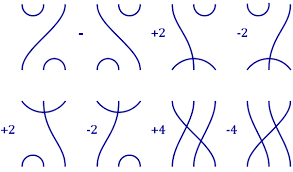
\includegraphics[width=0.5\textwidth]{../pics/Q3_on_MPS.png}
%
\caption[Graphical representation of $Q_{ijk}$ acting on a general $\ket{\text{MPS}}$]{Graphical representation of $Q_{ijk}$ acting on a general $\ket{\text{MPS}}$. The three indices $i$, $j$, $k$ are  all adjacent in $\text{MPS}^{i_1 \ldots i_{\ell} \ldots i_L}$. As can be seen from the picture, the different contributions do not in general cancel when we sum over $\ell$. This figure was taken from \cite{MPS bethe state overlap SO(5)}.}
%
\label{fig:Q3_on_MPS}
%
\end{center}
%
\end{figure}
%
%

\paragraph[The $SO(3)$ symmetric setup]{The $\mathbf{SO(3)}$ symmetric setup}
for this particular setup, the matrices $\mathcal{V}_i$ are just $SO(3)$ generators, and thus satisfy the commutation relations: $[\mathcal{V}_i, \mathcal{V}_j] = i \, \varepsilon_{ijk} \mathcal{V}^k$. We can use these commutation relations, and the fact that $\mathcal{V}_s \mathcal{V}^s = (k^2 - 1) / 4$, to further simplify the action of $Q_{\ell-1,\ell,\ell+1}$ on the MPS.
%
%
\begin{equation*}
(Q_{\ell-1,\ell,\ell+1} \cdot \text{MPS})_{ijk}
=
\frac{1}{4} \left(k^2 - 1 \right) \, \mathcal{V}_i \, \delta_{jk}
+
2 \, \mathcal{V}_i \, \delta_{jk}
+
4 \, i \, \mathcal{V}_i \, \varepsilon_{jks} \, \mathcal{V}^s
\end{equation*}
%
%
\begin{equation}
-
\frac{1}{4} \left(k^2 - 1 \right) \, \delta_{ij} \, \mathcal{V}_k
-
2 \, \delta_{ij} \, \mathcal{V}_k
-
4 \, i \, \varepsilon_{ijs} \, \mathcal{V}^s \mathcal{V}_k
\end{equation}
%
%
Upon summing over all $\ell$ and taking the trace over the $\mathcal{V}_{i_\ell}$ matrices, we find that the above expression vanishes. For example, if we focus on the terms $2 \, \mathcal{V}_i \, \delta_{jk}$ and $-2 \, \delta_{ij} \, \mathcal{V}_k$ in the above expression, and define $p \equiv i_{\ell+2}$, we see that.
%
%
\begin{equation}
\tr[ \cdots (2 \, \mathcal{V}_i \, \delta_{jk}) \, \mathcal{V}_p \cdots ]
+
\tr[ \cdots \mathcal{V}_i \, (-2 \, \delta_{jk} \, \mathcal{V}_p) \cdots ]
=
0
\end{equation}
%
%
\begin{figure}
%
\begin{center}
%
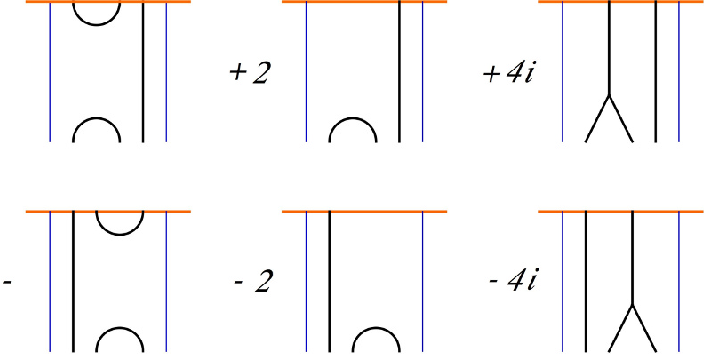
\includegraphics[width=0.7\textwidth]{../pics/Q3_on_MPS_SO(3).png}
%
\caption[Graphical representation of the action $Q_{ijk}$ on a $SO(3)$ sym. $\ket{\text{MPS}}$]{Graphical representation of the action $Q_{ijk}$ on $\ket{\text{MPS}}$, for a $SO(3)$ symmetric $\ket{\text{MPS}}$. The three indices $i$, $j$, $k$ are  all adjacent in $\text{MPS}^{i_1 \ldots i_{\ell} \ldots i_L}$. As can be seen from the picture, the different contributions can in this case be unravelled, an are seen to cancel when we sum over $\ell$. This figure was taken from \cite{MPS bethe state overlap}.}
%
\label{fig:Q3_on_MPS_simplified}
%
\end{center}
%
\end{figure}
%
%
The remaining four terms can analogously be paired up, and one finds that they will cancel each other in the same manner as in the example above. This cancelation can also be expressed graphically, as seen in figure \ref{fig:Q3_on_MPS_simplified}.

\newpage
\paragraph[The $SO(5)$ symmetric setup]{The $\mathbf{SO(5)}$ symmetric setup}
in this dCFT setup, the matrices $\mathcal{V}_i$ are now given by the subset $G_{i6}^{d_n}$, with $i=1,2,3,4,5$, of the $d_n$ dimensional representation of $SO(6)$ generators. The commutation relation between $\mathcal{V}_i$ matrices in this setup therefore takes the following form.
%
%
\begin{equation}
[\mathcal{V}_i, \mathcal{V}_j] = i \, G_{ij}^{d_n} \equiv i \, \mathcal{V}_{ij}
\end{equation}
%
%

%
%
\begin{equation}
\mathcal{V}_s \mathcal{V}^s
=
C_6 \left( \frac{n}{2}, \frac{n}{2}, \frac{n}{2} \right)
- C_5 \left( \frac{n}{2}, 0 \right)
=
\frac{n (n + 1)}{4}
\end{equation}
%
%
Where the matrices $G_{ij}^{d_n}$ represents the last $5 \cdot 4 / 2 = 10$ generators of $SO(6)$. For more information about the $SO(5)$ and $SO(6)$ Casimir operators, refer to appendix \ref{sec:so(5)_so(6)_rep_theory}. Using the above commutation relations together with the Casimir operator, we find that.
%
%
\begin{equation}
(Q_{\ell-1,\ell,\ell+1} \cdot \text{MPS})_{ijk}
=
\frac{1}{4} n (n + 4) \, (\delta_{ij} \, \mathcal{V}_k - \mathcal{V}_i \, \delta_{jk})
+
4 \, i \, (\mathcal{V}_{ij} \mathcal{V}_k - \mathcal{V}_i \mathcal{V}_{jk})
\end{equation}
%
%
Upon summing over all $\ell$ and taking the trace over the generator matrices, we again find that the MPS is annihilated by $Q_3$. The reasoning is exactly the same as in the $SO(3)$ symmetric case.

\paragraph[The $SO(3) \times SO(3)$ symmetric setup]{The $\mathbf{SO(3) \times SO(3)}$ symmetric setup}
for this case, the $\mathcal{V}_i$ matrices do not constitute a set of Lie algebra generators, and so do not satisfy any commutation relation which would help reduce (\ref{Q_3 piece on MPS general}). Thus, one would not expect the MPS to be annihilated by $Q_3$ in this particular dCFT setup, and this is indeed the case on spin-chains with $L \geq 12$ \cite{Lack of integrability in SO(3)xSO(3)}. 

\subsubsection{Tree-level Bethe operator one-point functions}
In the dCFT setups in which the MPS is annihilated by $Q_3$, we can now make use of the spin-chain formalism in order to obtain the tree-level contributions to Bethe state operators $\mathcal{O}_{\boldsymbol{L}}$. To do this, we need to first introduce the parity operator $\mathcal{P}$ of the spin-chain. In what follows, we label the sites of the spin-chain by $\ell = -\ell_L, -\ell_L + 1, \ldots , \ell_L - 1, \ell_L$, where $\ell_L = \lfloor \frac{L}{2} \rfloor$ and $\ell = 0$ is excluded for $L$ even. We define the parity operator $\mathcal{P}$ by its action on the basis states as follow.
%
%
\begin{equation}
\mathcal{P} \ket{\sigma_{-\ell_L} \sigma_{-\ell_L+1} \ldots \sigma_{\ell_L - 1} \sigma_{\ell_L}}
=
\ket{\sigma_{\ell_L} \sigma_{\ell_L-1} \ldots \sigma_{-\ell_L + 1} \sigma_{-\ell_L}}
\end{equation}
%
%
Using the above definition, we can now easily show that the conserved charge $Q_3$ is odd under parity.

\newpage
%
%
\begin{equation*}
\mathcal{P} \, Q_{\ell-1,\ell,\ell+1} \, \mathcal{P}^{-1}
=
Q_{-\ell+1, -\ell, -\ell-1}
=
[\mathcal{H}_{-\ell+1, -\ell}, \mathcal{H}_{-\ell, -\ell-1}]
\end{equation*}
%
%
\begin{equation}
=
-[\mathcal{H}_{-\ell-1, -\ell}, \mathcal{H}_{-\ell, -\ell+1}]
\end{equation}
%
%

%
%
\begin{equation}
\Rightarrow \quad
%
\mathcal{P} \, Q_3 \, \mathcal{P}^{-1}
=
\sum_{\ell}
\mathcal{P} \, Q_{\ell-1,\ell,\ell+1} \, \mathcal{P}^{-1}
=
-\sum_{\ell}
Q_{-\ell-1, -\ell, -\ell+1}
=
-Q_3
\end{equation}
%
%
Until this point  we have been referring to the eigenstates of the spin-chain as $\ket{\Psi_M}$. In what follows, it will however be convenient to be more precise and label the eigenstates by the rapidity parameters: $\ket{\{ u_j \}}$. Using (\ref{spin-chain momentum}) and the fact that the momentum operator is odd under parity, we find that.
%
%
\begin{equation}
\mathcal{P} \, P \, \mathcal{P}^{-1} = -P
%
\quad \Rightarrow \quad
%
\mathcal{P} \ket{\{ u_j \}} \sim \ket{\{ -u_j \}}
\end{equation}
%
%
From the above, we see that generally, an eigenstate of the spin-chain gets mapped to a different eigenstates with opposite momentum. For the special case of so-called \textit{unpaired states}, where the rapidity parameters come in opposite sign pairs, the parity operator only multiplies by a factor. In other words, the states of the form $\ket{\{ u_j , -u_j \}}$ are eigenstates of the parity operator. This implies.
%
%
\begin{equation}
Q_3 \ket{\{ u_j, -u_j \}} = q_3 \ket{\{ u_j, -u_j \}}
%
\quad \Rightarrow \quad
%
Q_3 \ket{\{ u_j, -u_j \}} = -q_3 \ket{\{ u_j, -u_j \}}
\end{equation}
%
%
Thus we conclude that $q_3 = 0$ for unpaired states. Moreover, it can be seen from the explicit form of the $Q_3$ eigenvalues, that all spin-chain eigenstates which are not unpaired, will have $q_3 \neq 0$ \cite{Conserved charges eigenvalues}.
%
%
\begin{equation}
Q_3 = \frac{i}{2} \left. \frac{d^2}{du^2} F(u) \right|_{i=i/2}
\end{equation}
%
%
\begin{equation}
Q_3 \ket{\Psi_M} = \sum_{j=1}^M q_3(u_j) \ket{\Psi_M}
%
\quad , \quad
%
q_3(u_j) = \frac{i}{2}
\left[ \frac{1}{(u_j + i/2)^2} - \frac{1}{(u_j - i/2)^2} \right]
\end{equation}
%
%
This means that all Bethe state operators $\mathcal{O}_{\boldsymbol{L}}(x)$ which do not correspond to unpaired states will vanish at tree-level, since.
%
%
\begin{equation}
0 = \bra{\text{MPS}} Q_3 \ket{ \{ u_j \} }
= q_3 \braket{\text{MPS}}{ \{ u_j \} }
%
\quad \Rightarrow \quad
%
\braket{\text{MPS}}{ \{ u_j \} } = 0
\end{equation}
%
%
Where we have used that the MPS is annihilated by $Q_3$. Thus, we can focus on overlaps between the MPS and unpaired Bethe states. Furthermore, it can be shown that the overlap between the MPS and a given Bethe state $\ket{\Psi_M}$, vanishes unless both $L$ and $M$ are even \cite{MPS bethe state overlap}.\\
Using the spin-chain picture, and all the insight which can be extracted from this approach, it is possible to find tree-level expressions for one-point functions of the Bethe state type. For example, in the case of the $SO(3)$ symmetric defect setup, the tree-level contribution to $\expval{\mathcal{O}_{\boldsymbol{L}}(x)}$ can be written as follow \cite{MPS bethe state overlap, non-protected one-point functions}.
%
%
\begin{equation}
SO(3) : \quad
%
\expval{\mathcal{O}_{\boldsymbol{L}}(x)}_{\text{tree}}
=
\frac{C_k(\{ u_j \})}{x_3^L}
\end{equation}
%
%
Where $C_k(\{ u_j \})$ is given by the following expression.
%
%
\begin{equation}
C_k(\{ u_j \})
=
2^{L-1} C_2(\{ u_j \})
\sum_{j=\frac{1-k}{2}}^{\frac{k-1}{2}}
j^L
\prod_{i=1}^{\frac{M}{2}}
\frac{u_i^2 \left(u_i^2 + \frac{k^2}{4} \right)}
{\left[ u_i^2 + \left(j - \frac{1}{2} \right)^2 \right]
\left[ u_i^2 + \left(j + \frac{1}{2} \right)^2 \right]}
\end{equation}
%
%
And $C_2(\{ u_j \})$ is given by the expression.
%
%
\begin{equation}
C_2(\{ u_j \})
=
2 \left[
\left( \frac{2 \pi^2}{\lambda} \right)^L
\frac{1}{L}
\prod_{j=1}^M
\frac{u_j^2 + \frac{1}{4}}{u_j^2}
\frac{\det G^{+}}{\det G^{-}}
\right]^{1 / 2}
\end{equation}
%
%
And lastly, the $\frac{M}{2} \times \frac{M}{2}$ matrices $G^{\pm}$ are given by the expression.
%
%
\begin{equation}
G_{jk}^{\pm} 
=
\left(
\frac{L}{u_j^2 + \frac{1}{4}}
-
\sum_{n=1}^{\frac{M}{2}}
K_{jn}^{+}
\right)
\delta_{jk}
+
K_{jk}^{\pm}
\end{equation}
%
%
\begin{equation}
K_{jk}^{\pm}
=
\frac{2}{1 + (u_j - u_k)^2}
\pm
\frac{2}{1 + (u_j + u_k)^2}
\end{equation}
%
%
In the cases of the $SO(3) \times SO(3)$ symmetric defect setup, a general expression for the tree-level contribution to Bethe state one-point functions are not yet known at the time of writing this thesis. However, for special values of parameters, such as $L$ and $M$, results are known for the $SO(3) \times SO(3)$ symmetric setup \cite{Lack of integrability in SO(3)xSO(3)}. For the case of the $SO(5)$ symmetric defect setup, a general closed expression was recently found in \cite{Overlap SO(5) general formula}.\\
This concludes our discussion of how to include defects into the spin-chain picture using the MPS, and how these states in some cases can be used to find explicit expressions for tree-level contributions to Bethe state one-point functions. In the next subsection, we will discuss how we can use these results to find tree-level contributions to the long / short two-point functions $\expval{\mathcal{O}_L \mathcal{O}_{W_1 W_2}}$ described at the beginning of this section. 

\newpage
\subsection{Computing the long / short two-point functions}
In this subsection, we finally begin to tackle the central problem layed out at the start of this section; namely how to compute the leading order connected contribution to two-point functions of the form.
%
%
\begin{equation*}
\expval{\mathcal{O}_{\boldsymbol{L}}(x) \mathcal{O}_{\boldsymbol{W}_1 \boldsymbol{W}_2}(y)}
=
\contraction{\sum_{\ell=1}^L \Psi_M^{i_1 \cdots i_L} 
\tr \big[ \mathcal{V}_{i_1} \cdots }
{V_{i_\ell}}
{ \cdots \mathcal{V}_{i_L} \big] \tr \big[ }
{W_1}
\sum_{\ell=1}^L \Psi_M^{i_1 \cdots i_L} 
\tr \big[ \mathcal{V}_{i_1} \cdots V_{i_\ell} \cdots \mathcal{V}_{i_L} \big] 
\tr \big[ W_1 \mathcal{W}_2 \big]
\end{equation*}
%
%
\begin{equation}\label{The_Two_Point_Function}
+
(W_1 \leftrightarrow W_2)
\end{equation}
%
%
In the above expression, $V_{i_\ell} \in \{ X, Z \}$ and $W_1, W_2 \in \{ X,Y,Z,\bar{X},\bar{Y},\bar{Z} \}$. We will postpone the discussion of the cases $W_1 \in \{ Y,\bar{Y} \}$ or $W_2 \in \{ Y,\bar{Y} \}$ untill the end of this subsection, as these require a slightly different treatment, for reason which will hopefully become clear later on. It should be noted at this point, that our method for computing the two-point functions \ref{The_Two_Point_Function} has been greatly inspired by the work presented in \cite{Length L length 2 two-point functions D5-D3}, in which two-point functions of the form \ref{The_Two_Point_Function} are evaluated in the $SO(3)$ symmetric D5-D3 probe brane setup.

\subsubsection[$SO(3) \times SO(3)$ symmetric vevs]{$\mathbf{SO(3) \times SO(3)}$ symmetric vevs}
As an intermediate step in the process of computing these two-point funtions, we will be interested in all operators of the form.
%
%
\begin{equation}\label{The T operators}
T_{V_{i_\ell} W_1 W_2}
\equiv
\contraction{}
{V_{i_\ell}}
{ \tr \big[ }
{W_1}
V_{i_\ell} \tr \big[ W_1 \mathcal{W}_2 \big]
=
\hat{Y}_{\ell_1}^{m_1} \otimes \hat{Y}_{\ell_2}^{m_2}
\tr[\hat{Y}_{\ell_1'}^{m_1'} \otimes \hat{Y}_{\ell_2'}^{m_2'} \, \mathcal{W}_2]
\expval{[V_{i_{\ell}}]_{\boldsymbol{\ell}} \, [W_1]_{\boldsymbol{\ell}'}}
\end{equation}
%
%
Where we have used the $\boldsymbol{\ell} = (\ell_1, m_1; \ell_2, m_2)$ introduced in earlier sections. Looking at the form of (\ref{The_Two_Point_Function}), the motivation for why one would be interested in the $T$ operators should be fairly obvious. A priori, there seem to be a large number of different $T$ operators, but fortunately it turns out that the forms of all $T$ operators can be infered from just a few specific cases, as we shall now see.

\paragraph[The $T$ operators: ideas and examples]{The $\mathbf{T}$ operators: ideas and examples}
Before we start the process of computing the $T$ operators, let us first make some simplifying redefinitions of some of the objects in (\ref{The T operators}). These redefinitions looks as follow.
%
%
\begin{equation}\label{rescaling of T objects}
\expval{[V_{i_{\ell}}]_{\boldsymbol{\ell}} \, [W_1]_{\boldsymbol{\ell}'}}
\to
x_3 y_3 \expval{[V_{i_{\ell}}]_{\boldsymbol{\ell}} \, [W_1]_{\boldsymbol{\ell}'}}
%
\quad , \quad
%
\mathcal{V}_{i_\ell} \to x_3 \, \mathcal{V}_{i_\ell}
%
\quad , \quad
%
\mathcal{W}_{1,2} \to y_3 \, \mathcal{W}_{1,2}
\end{equation}
%
%
These rescalings exactly cancel the spacetime dependence of the objects being rescaled, and thus the $T$ operators all become spacetime independent after these rescalings. If need be, we can always recover the spacetime dependence of any $T$ operator by undoing \ref{rescaling of T objects}.

\subparagraph[The operator $T_{ZZZ}$]{The operator $\mathbf{T_{ZZZ}}$:} Let us, somewhat arbitrarily, take this specific $T$ operator to be the starting point in our process of computing all $T$ operators. According to (\ref{The T operators}), $T_{ZZZ}$ is given as follow.
%
%
\begin{equation}
T_{ZZZ} = \hat{Y}_{\ell_1}^{m_1} \otimes \hat{Y}_{\ell_2}^{m_2}
\tr[\hat{Y}_{\ell_1'}^{m_1'} \otimes \hat{Y}_{\ell_2'}^{m_2'} \, \mathcal{Z}]
\expval{Z_{\ell_1, m_1; \ell_2, m_2} \, Z_{\ell_1', m_1'; \ell_2', m_2'}}
\end{equation}
%
%
In order to compute the trace, we take advantage of the orthogonality of the fuzzy spherical harmonics, together with relation between $t_3^k$, $\mathbb{1}_k$ and the fuzzy spherical harmonics $\hat{Y}_{\ell}^{m}$. We restate these relations below for convenience.
%
%
\begin{equation}\label{orthogonality}
\tr[\hat{Y}_{\ell}^{m} \, \hat{Y}_{\ell'}^{m'}]
=
(-1)^{m'} \delta_{\ell, \ell'} \, \delta_{m + m',0}
\end{equation}
%
%
\begin{equation}
\mathbb{1} = d_0^k \, \hat{Y}^{0}_{0}
%
\quad , \quad
%
t_3 = \sqrt{2} \, d_1^k \, \hat{Y}^{0}_{1}
\end{equation}
%
%
\begin{equation}
d_0^k = (-1)^{k+1} \sqrt{k}
%
\quad , \quad
%
d_1^k = \frac{(-1)^{k+1}}{2} \sqrt{\frac{k(k^2-1)}{6}}
\end{equation}
%
%
Using the above information, we can evaluate the trace appearing in $T_{ZZZ}$, which yields the result.
%
%
\begin{equation*}
\tr[\hat{Y}_{\ell_1'}^{m_1'} \otimes \hat{Y}_{\ell_2'}^{m_2'} \, \mathcal{Z}]
=
\tr[\hat{Y}_{\ell_1'}^{m_1'} \, t_3^{k_1} \otimes \hat{Y}_{\ell_2'}^{m_2'} ]
+
i \tr[\hat{Y}_{\ell_1'}^{m_1'} \otimes \hat{Y}_{\ell_2'}^{m_2'} \, t_3^{k_2} ]
\end{equation*}
%
%
\begin{equation}\label{Z-trace}
=
\sqrt{2} \, d_1^{k_1} \, \delta_{\ell_1',1} \, \delta_{m_1',0} \,
d_0^{k_2} \, \delta_{\ell_2',0} \, \delta_{m_2',0}
+
i \, d_0^{k_1} \, \delta_{\ell_1',0} \, \delta_{m_1',0} \, 
\sqrt{2} \, d_1^{k_2} \, \delta_{\ell_2',1} \, \delta_{m_2',0}
\end{equation}
%
%
Now, let us turn our attention to propagator appearing in $T_{ZZZ}$. The propagator is between $Z$-fields, which makes it particularly simple. We restate the form of the $ZZ$-propagator below for convenience.
%
%
\begin{equation}
\expval{
Z_{\ell_1,m_1;\ell_2,m_2}
Z_{\ell_1',m_1';\ell_2',m_2'}
}
=
(-1)^{m_1' + m_2'}
\delta_{\ell_1 \ell_1'} \delta_{\ell_2 \ell_2'}
\delta_{m_1+m_1',0} \delta_{m_2 + m_2',0}
K^{ZZ}
\end{equation}
%
%

%
%
\begin{equation}
K^{ZZ}
=
\left[
K^{\phi,(1)}_{\mathrm{sing}} - K^{\phi,(2)}_{\mathrm{sing}}
- m_1^2 \, K^{\phi,(1)}_{\mathrm{sym}}
+ m_2^2 \, K^{\phi,(2)}_{\mathrm{sym}}
+ 2i \, m_1 m_2 \, K^{\phi}_{\mathrm{opp}}
\right]
\end{equation}
%
%
The exact expressions for the different $K$'s can be found in appendix \ref{app:complex propagators}, and also in \cite{One-point functions in D3-D7}. Now that we have computed the trace and re-familiarized ourselves with the form of the $ZZ$-propagator, we are ready to simplify the form of the operator $T_{ZZZ}$. All terms in $K^{ZZ}$ proportional to $m_1$ or $m_2$ drop out due to the $\delta$-symbols, and we are left with the following expression.
%
%
\begin{equation*}
T_{ZZZ}
=
\sqrt{2} \, d_1^{k_1} \, d_0^{k_2} \, \hat{Y}^{0}_{1} \otimes \hat{Y}^{0}_{0}
\left[
K^{\phi,(1)}_{\mathrm{sing}} - K^{\phi,(2)}_{\mathrm{sing}}
\right]_{\ell_1=1,\ell_2=0}
\end{equation*}
%
%
\begin{equation*}
+
i \, \sqrt{2} \, d_0^{k_1} \, d_1^{k_2} \, \hat{Y}^{0}_{0} \otimes \hat{Y}^{0}_{1}
\left[
K^{\phi,(1)}_{\mathrm{sing}} - K^{\phi,(2)}_{\mathrm{sing}}
\right]_{\ell_1=0,\ell_2=1}
\end{equation*}
%
%
\begin{equation}
=
\frac{1}{3}
\left(
2 K^{m^2 = 0}
- 3 K^{m^2 = 2}
+ K^{m^2 = 6}
\right)
\bar{\mathcal{Z}}
\end{equation}
%
%
Where we have used the following information.
%
%
\begin{equation}
\ell_1 = 1 \; , \; \ell_2 = 0 : \quad
%
K^{\phi,(1)}_{\mathrm{sing}}
=
\frac{2}{3} \, K^{m^2 = 0}
+
\frac{1}{3} \, K^{m^2 = 6}
%
\quad , \quad
%
K^{\phi,(2)}_{\mathrm{sing}}
=
K^{m^2 = 2}
\end{equation}
%
%
\begin{equation}
\ell_1 = 0 \; , \; \ell_2 = 1 : \quad
%
K^{\phi,(2)}_{\mathrm{sing}}
=
\frac{2}{3} \, K^{m^2 = 0}
+
\frac{1}{3} \, K^{m^2 = 6}
%
\quad , \quad
%
K^{\phi,(1)}_{\mathrm{sing}}
=
K^{m^2 = 2}
\end{equation}
%
%
In order to obtain the last equality. Note that $T_{ZZZ} \sim \mathcal{\bar{Z}}$. This turns out to be an important observation.

\subparagraph[The operator $T_{XZZ}$]{The operator $\mathbf{T_{XZZ}}$:} this $T$ operator is very similar in form to the $T_{ZZZ}$ operator. The trace which appears in the operator is the same as for $T_{ZZZ}$, but the propagator is now of $XZ$-type, as seen below.
%
%
\begin{equation}
T_{XZZ} = \hat{Y}_{\ell_1}^{m_1} \otimes \hat{Y}_{\ell_2}^{m_2}
\tr[\hat{Y}_{\ell_1'}^{m_1'} \otimes \hat{Y}_{\ell_2'}^{m_2'} \, \mathcal{Z}]
\expval{X_{\ell_1, m_1; \ell_2, m_2} \, Z_{\ell_1', m_1'; \ell_2', m_2'}}
\end{equation}
%
%
Seeing as we just evaluated the trace appearing in $T_{XZZ}$, all we need is the form of the $XZ$-propagator, before we can begin to simplify. We restate the form of the $XZ$-propagator below for convenience.
%
%
\begin{equation*}
\expval{
X_{\ell_1,m_1;\ell_2,m_2}
Z_{\ell_1',m_1';\ell_2',m_2'}
}
=
(-1)^{m_1' + m_2'} \delta_{\ell_1 \ell_1'} \delta_{\ell_2 \ell_2'}
\end{equation*}
%
%
\begin{equation*}
\times
\Bigg[
\delta_{m_2 + m_2',0}
\left(
i [t_2^{k_1}]_{m_1,-m_1'} K^{\phi,(1)}_{\text{anti}}
- [t_1^{k_1} t_3^{k_1}]_{m_1,-m_1'} K^{\phi,(1)}_{\text{sym}}
\right)
\end{equation*}
%
%
\begin{equation*}
-
\delta_{m_1 + m_1',0}
\left(
i [t_2^{k_2}]_{m_2,-m_2'} K^{\phi,(2)}_{\text{anti}}
- [t_1^{k_2} t_3^{k_2}]_{m_2,-m_2'} K^{\phi,(2)}_{\text{sym}}
\right)
\end{equation*}
%
%
\begin{equation}\label{XZ-propagator}
+
i
\left(
[t_1^{k_2}]_{m_2,-m_2'} [t_3^{k_1}]_{m_1,-m_1'}
+
[t_1^{k_1}]_{m_1,-m_1'} [t_3^{k_2}]_{m_2,-m_2'}
\right)
K^{\phi}_{\text{opp}}
\Bigg]
\end{equation}
%
%
Where in the above, the matrix representations of the different $\mathfrak{su}(2)$ generators are given as follow.
%
%
\begin{equation}\label{t1-rep}
[t_1]_{m,m'} = \frac{1}{2} \left(
\sqrt{(\ell+m)(\ell-m')} \, \delta_{m',m-1}
+
\sqrt{(\ell+m')(\ell-m)} \, \delta_{m',m+1}
\right)
\end{equation}
%
%
\begin{equation}\label{t2-rep}
[t_2]_{m,m'} = \frac{1}{2 \, i} \left(
\sqrt{(\ell+m)(\ell-m')} \, \delta_{m',m-1}
-
\sqrt{(\ell+m')(\ell-m)} \, \delta_{m',m+1}
\right)
\end{equation}
%
%
\begin{equation}\label{t3-rep}
[t_3]_{m,m'} = m' \, \delta_{m,m'}
\end{equation}
%
%
\begin{equation}
[t_1 t_3]_{m,m'} = [t_1]_{m,m''} [t_3]_{m'',m'} = m' \, [t_1]_{m,m'}
\end{equation}
%
%
Now that we know the form of the $XZ$-propagator, we are ready to simplify the $T_{XZZ}$ operator. Using the trace result (\ref{Z-trace}) and propagator form (\ref{XZ-propagator}), we can make some immediate simplifications.
%
%
\begin{enumerate}
%
\item Since the $k=1$ representation of $\mathfrak{su}(2)$ is trivial, meaning that $t^{k=1}_i = 0$, all terms containing either $\delta_{\ell_1,0} \, t_i^{k_1}$ or $\delta_{\ell_2,0} \, t_i^{k_2}$ will vanish.
%
\item It turns out that the propagators $K^{\phi,(1)}_{\text{sym}}$ and $K^{\phi,(2)}_{\text{sym}}$, vanish for the cases $\ell_1=1$, $\ell_2=0$ and $\ell_1=0$, $\ell_2=1$ respectively. The explicit forms of $K^{\phi,(1)}_{\text{sym}}$ and $K^{\phi,(2)}_{\text{sym}}$ can be found in appendix \ref{app:complex propagators} and in \cite{One-point functions in D3-D7}.
%
\end{enumerate}
%
%
Using the above information, we see that the $2 \times 6$ terms constituting $T_{XZZ}$ collapses down to only 2. 
%
%
\begin{equation*}
T_{XZZ}
=
-\frac{1}{2} \sqrt{2} \, d_1^{k_1} \, d_0^{k_2} \left[
\hat{Y}^{-1}_{1} \otimes \hat{Y}^{0}_{0}
-
\hat{Y}^{1}_{1} \otimes \hat{Y}^{0}_{0}
\right]
\left. K^{\phi,(1)}_{\text{anti}} \right|_{\ell_1=1,\ell_2=0}
\end{equation*}
%
%
\begin{equation*}
+ i \, \frac{1}{2} \sqrt{2} \, d_0^{k_1} \, d_1^{k_2}\left[
\hat{Y}^{0}_{0} \otimes \hat{Y}^{-1}_{1}
-
\hat{Y}^{0}_{0} \otimes \hat{Y}^{1}_{1}
\right]
\left. K^{\phi,(2)}_{\text{anti}} \right|_{\ell_1=0,\ell_2=1}
\end{equation*}
%
%
\begin{equation}
=
-\frac{1}{3} \left(
K^{m^2=0} - K^{m^2=6}
\right)
\bar{\mathcal{X}}
\end{equation}
%
%
Where we have used the following information.
%
%
\begin{equation}
\ell_1 = 1 \; , \; \ell_2 = 0 : \quad
%
K^{\phi,(1)}_{\mathrm{anti}}
=
\frac{1}{3} \, K^{m^2 = 0}
-
\frac{1}{3} \, K^{m^2 = 6}
\end{equation}
%
%
\begin{equation}
\ell_1 = 0 \; , \; \ell_2 = 1 : \quad
%
K^{\phi,(2)}_{\mathrm{anti}}
=
\frac{1}{3} \, K^{m^2 = 0}
-
\frac{1}{3} \, K^{m^2 = 6}
\end{equation}
%
%
In order to obtain the last equality. Once again, we see that the result after simplification is proportional to a single complex classical scalar. This time we find $T_{XZZ} \sim \mathcal{\bar{X}}$.

\subparagraph[The operator $T_{ZXZ}$]{The operator $\mathbf{T_{ZXZ}}$:} we now encounter our first example that the form of one $T$ operator can be infered from another. The unsimplified form of $T_{ZXZ}$ is given by the following expression.
%
%
\begin{equation}
T_{ZXZ} = \hat{Y}_{\ell_1}^{m_1} \otimes \hat{Y}_{\ell_2}^{m_2}
\tr[\hat{Y}_{\ell_1'}^{m_1'} \otimes \hat{Y}_{\ell_2'}^{m_2'} \, \mathcal{Z}]
\expval{Z_{\ell_1, m_1; \ell_2, m_2} \, X_{\ell_1', m_1'; \ell_2', m_2'}}
\end{equation}
%
%
As can be seen from the above expression, $T_{ZXZ}$ is almost exactly identical to $T_{XZZ}$. The only difference is that $X$ and $Z$ are switched in the propagator. It turns out that the $ZX$-propagator can be obtained from the $XZ$-propagator by making the substitutions $t_1 \to t_3$, $t_3 \to t_1$ and $t_2 \to - t_2$. This can be seen from the generic expression for the $\phi_i$ propagators, which can be found in either appendix \ref{app:complex propagators} or \cite{One-point functions in D3-D7}. Thus, we find that the operator $T_{ZXZ}$ can be written as.
%
%
\begin{equation}
T_{ZXZ} = \frac{1}{3} \left(
K^{m^2=0} - K^{m^2=6}
\right)
\bar{\mathcal{X}}
\end{equation}
%
%
Since all the terms containing $t_1$ and $t_3$ vanish for the same reasons as in the $T_{XZZ}$ operator case.

\subparagraph[The operator $T_{ZZX}$]{The operator $\mathbf{T_{ZZX}}$:} this operator is again one which cannot be infered from any $T$ operator we have alreday computed. More work is once again needed. The explicit un-simplified expression for $T_{ZZX}$ looks as follow.
%
%
\begin{equation}
T_{ZZX} = \hat{Y}_{\ell_1}^{m_1} \otimes \hat{Y}_{\ell_2}^{m_2}
\tr[\hat{Y}_{\ell_1'}^{m_1'} \otimes \hat{Y}_{\ell_2'}^{m_2'} \, \mathcal{X}]
\expval{Z_{\ell_1, m_1; \ell_2, m_2} \, Z_{\ell_1', m_1'; \ell_2', m_2'}}
\end{equation}
%
%
To compute the trace, we take advantage of the orthogonality of the fuzzy spherical harmonics (\ref{orthogonality}), together with the expasion of $t_1$ in terms of the fuzzy spherical harmonics.
%
%
\begin{equation}
t_1 = d_1^k \left( \hat{Y}^{-1}_{1} - \hat{Y}^{1}_{1} \right)
%
\quad , \quad
%
d_1^k = \frac{(-1)^{k+1}}{2} \sqrt{\frac{k(k^2-1)}{6}}
\end{equation}
%
%
Using the above information, we can now evaluate the trace appearing in $T_{ZZX}$. The result is this.
%
%
\begin{equation*}
\tr[\hat{Y}_{\ell_1'}^{m_1'} \otimes \hat{Y}_{\ell_2'}^{m_2'} \mathcal{X}]
=
\tr[\hat{Y}_{\ell_1'}^{m_1'} t_1^{k_1} \otimes \hat{Y}_{\ell_2'}^{m_2'} ]
+
i \tr[\hat{Y}_{\ell_1'}^{m_1'} \otimes \hat{Y}_{\ell_2'}^{m_2'} t_1^{k_2} ]
\end{equation*}
%
%
\begin{equation*}
=
d_1^{k_1} \, \delta_{\ell_1',1} \, (\delta_{m_1',-1} - \delta_{m_1',1}) \,
d_0^{k_2} \, \delta_{\ell_2',0} \, \delta_{m_2',0}
\end{equation*}
%
%
\begin{equation}
+
i \, d_0^{k_1} \, \delta_{\ell_1',0} \, \delta_{m_1',0}
\, d_1^{k_2} \, \delta_{\ell_2',1} \, (\delta_{m_2',-1} - \delta_{m_2',1})
\end{equation}
%
%
Now that we have computed the trace, we are ready to simplify the form of the operator $T_{ZZX}$. The terms in $K^{ZZ}$ proportional to $m_2$ drops out when multiplied by the first term of the above trace, and the terms proportional to $m_1$ drops out when multiplied by the second term of the trace. Furthermore, we found earlier on that $K^{\phi,(1)}_{\text{sym}} |_{\ell_1=1,\ell_2=0} = K^{\phi,(2)}_{\text{sym}} |_{\ell_1=0,\ell_2=1} = 0$. Using this information, we obtain the following simplified expression for $T_{ZZX}$.
%
%
\begin{equation*}
T_{ZZX}
=
d_1^{k_1} \, d_0^{k_2} \left(
\hat{Y}^{-1}_{1} \otimes \hat{Y}^{0}_{0}
-
\hat{Y}^{1}_{1} \otimes \hat{Y}^{0}_{0}
\right)
\left[
K^{\phi,(1)}_{\mathrm{sing}} - K^{\phi,(2)}_{\mathrm{sing}}
\right]_{\ell_1=1,\ell_2=0}
\end{equation*}
%
%
\begin{equation*}
+
i \, d_0^{k_1} \, d_1^{k_2} \left(
\hat{Y}^{0}_{0} \otimes \hat{Y}^{-1}_{1}
-
\hat{Y}^{0}_{0} \otimes \hat{Y}^{1}_{1}
\right)
\left[
K^{\phi,(1)}_{\mathrm{sing}} - K^{\phi,(2)}_{\mathrm{sing}}
\right]_{\ell_1=0,\ell_2=1}
\end{equation*}
%
%
\begin{equation}\label{T_ZZX}
=
\frac{1}{3}
\left(
2 K^{m^2 = 0}
- 3 K^{m^2 = 2}
+ K^{m^2 = 6}
\right)
\bar{\mathcal{X}}
\end{equation}
%
%
It turns out that the $T$ operator above was the last one we need to compute explicitly. The rest of the $T$ operators can be inferred from the ones we already know, as we will now proceed to show.

\subparagraph[The operator $T_{XXZ}$]{The operator $\mathbf{T_{XXZ}}$:} this particular operator can be obtained from $T_{ZXX}$ by use of a similarity transformation. This transformation is an fact the exact same one we made use of back in section \ref{sec:CPO}. The transformation sends $t_1 \to t_3$, $t_2 \to -t_2$ and $t_3 \to t_1$, and is defined as follow.
%
%
\begin{equation}\label{similarity transform 1}
V = U^{k_1} \otimes U^{k_2}
%
\quad , \quad
%
U^{k_s} = e^{i \pi t_3^{k_s}} \, e^{i \pi t_2^{k_s} / 2}
\end{equation}
%
%
Using the following transformation properties of the fuzzy spherical harmonics and $\mathfrak{su}(2)$ generators.
%
%
\begin{equation}
U \, \hat{Y}^m_\ell \, U^\dagger
=
U_{n,m} \, \hat{Y}^n_\ell
%
\quad , \quad
%
U \, (\hat{Y}^m_\ell)^{\dagger} \, U^\dagger
=
\bar{U}_{n,m} \, \hat{Y}^n_\ell
%
\quad , \quad
%
U_{m,m'} = \bra{m} U \ket{m'}
\end{equation}
%
%
\begin{equation}
U_{m,n} \, \bar{U}_{m',n'} \, [t_3]_{n,n'} = [t_1]_{m,m'}
%
\quad , \quad
%
U_{m,n} \, \bar{U}_{m',n'} \, [t_1]_{n,n'} = [t_3]_{m,m'}
\end{equation}
%
%
We can now prove that $T_{XXZ}$ can be obtained from $T_{ZZX}$. Transforming $T_{ZZX}$ using $V$, we find that.
%
%
\begin{equation*}
V \, T_{ZZX} \, V^\dagger
=
V \, \hat{Y}_{\ell_1}^{m_1} \otimes \hat{Y}_{\ell_2}^{m_2} \, V^\dagger
\tr[V \, \hat{Y}_{\ell_1'}^{m_1'} \otimes \hat{Y}_{\ell_2'}^{m_2'} V^\dagger \, V \, \mathcal{X} \, V^\dagger]
\expval{Z_{\boldsymbol{\ell}} \, Z_{\boldsymbol{\ell}'}}K^{\phi,(1)}_{\mathrm{anti}}
\end{equation*}
%
%
\begin{equation*}
=
\hat{Y}_{\ell_1}^{n_1} \otimes \hat{Y}_{\ell_2}^{n_2}
\tr[\hat{Y}_{\ell_1'}^{n_1'} \otimes \hat{Y}_{\ell_2'}^{n_2'} \, \mathcal{Z}] \,
U^{k_1}_{n_1,m_1} \, U^{k_2}_{n_2,m_2} \,
\bar{U}^{k_1}_{-n_1',-m_1'} \, \bar{U}^{k_2}_{-n_2',-m_2'} \,
(-1)^{m_1' + m_2'}
\end{equation*}
%
%
\begin{equation}
\times
(-1)^{n_1' + n_2'} \,
\expval{Z_{\boldsymbol{\ell}} \, Z_{\boldsymbol{\ell}'}}
=
\hat{Y}_{\ell_1}^{n_1} \otimes \hat{Y}_{\ell_2}^{n_2}
\tr[\hat{Y}_{\ell_1'}^{n_1'} \otimes \hat{Y}_{\ell_2'}^{n_2'} \, \mathcal{Z}] \,
\expval{X_{\boldsymbol{\ell}} \, X_{\boldsymbol{\ell}'}}
=
T_{XXZ}
\end{equation}
%
%
We can now obtain the simplified form of $T_{XXZ}$, simply by transforming the result we already found for $T_{ZZX}$, using the $V$. The result is the following.
%
%
\begin{equation}
T_{XXZ} = \frac{1}{3}
\left(
2 K^{m^2 = 0}
- 3 K^{m^2 = 2}
+ K^{m^2 = 6}
\right)
\bar{\mathcal{Z}}
\end{equation}
%
%

\subparagraph[The operator $T_{XZX}$]{The operator $\mathbf{T_{XZX}}$:} this operator can by infered from the operator $T_{ZXZ}$, again by use of the similarity transformation $V$. The explicit unsimplified form of $T_{XZX}$ looks as follow.
%
%
\begin{equation}
T_{XZX} = \hat{Y}_{\ell_1}^{m_1} \otimes \hat{Y}_{\ell_2}^{m_2}
\tr[\hat{Y}_{\ell_1'}^{m_1'} \otimes \hat{Y}_{\ell_2'}^{m_2'} \, \mathcal{X}]
\expval{X_{\ell_1, m_1; \ell_2, m_2} \, Z_{\ell_1', m_1'; \ell_2', m_2'}}
\end{equation}
%
%
Transforming $T_{ZXZ}$ using $V$, we find that $T_{XZX}$ is given by the following simple expression.
%
%
\begin{equation}
T_{XZX} = \frac{1}{3} \left(
K^{m^2=0} - K^{m^2=6}
\right)
\bar{\mathcal{Z}}
\end{equation}
%
%

\paragraph[The $T$ operators: obtaining the rest]{The $\mathbf{T}$ operators: obtaining the rest}
It is now time to use the insight we have gained from computing a few of the $T$ operators, to infer the forms of the rest. First, we look at how to extend the results we found for $T_{ZZZ}$ and $T_{ZZX}$. Given the expression for the $Z \bar{Z}$-propagator.
%
%
\begin{equation}
\expval{
Z_{\ell_1,m_1;\ell_2,m_2}
\bar{Z}_{\ell_1',m_1';\ell_2',m_2'}
}
=
\delta_{\ell_1,\ell_1'} \, \delta_{\ell_2,\ell_2'} \,
\delta_{m_1,m_1'} \, \delta_{m_2,m_2'} \, K^{Z\bar{Z}}
\end{equation}
%
%
\begin{equation}
K^{Z\bar{Z}} =
\left[
K^{\phi,(1)}_{\mathrm{sing}} + K^{\phi,(2)}_{\mathrm{sing}}
- m_1^2 \, K^{\phi,(1)}_{\mathrm{sym}}
- m_2^2 \, K^{\phi,(2)}_{\mathrm{sym}}
\right]
\end{equation}
%
%
It is relatively easy to obtain the following results, by extend the results found for $T_{ZZZ}$ and $T_{ZZX}$.
%
%
\begin{equation}
T_{Z\bar{Z}Z} = \frac{1}{3}
\left(
2 K^{m^2 = 0}
+ 3 K^{m^2 = 2}
+ K^{m^2 = 6}
\right)
\mathcal{Z}
\end{equation}
%
%
\begin{equation}
T_{Z\bar{Z}X} =  \frac{1}{3}
\left(
2 K^{m^2 = 0}
+ 3 K^{m^2 = 2}
+ K^{m^2 = 6}
\right)
\mathcal{X}
\end{equation}
%
%
\begin{equation}
T_{Z\bar{Z}\bar{Z}} = \frac{1}{3}
\left(
2 K^{m^2 = 0}
+ 3 K^{m^2 = 2}
+ K^{m^2 = 6}
\right)
\bar{\mathcal{Z}}K^{\phi,(1)}_{\mathrm{anti}}
\end{equation}
%
%
\begin{equation}
T_{Z\bar{Z}\bar{X}} =  \frac{1}{3}
\left(
2 K^{m^2 = 0}
+ 3 K^{m^2 = 2}
+ K^{m^2 = 6}
\right)
\bar{\mathcal{X}}
\end{equation}
%
%
\begin{equation}
T_{ZZ\bar{Z}} = \frac{1}{3}
\left(
2 K^{m^2 = 0}
- 3 K^{m^2 = 2}
+ K^{m^2 = 6}
\right)
\mathcal{Z}
\end{equation}
%
%
\begin{equation}
T_{ZZ\bar{X}} =  \frac{1}{3}
\left(
2 K^{m^2 = 0}
- 3 K^{m^2 = 2}
+ K^{m^2 = 6}
\right)
\mathcal{X}
\end{equation}
%
%
If we look back at the computations of $T_{ZZZ}$ and $T_{ZZX}$, we see that only the $K^{\phi,(1)}_{\mathrm{sing}}$ and $K^{\phi,(2)}_{\mathrm{sing}}$ terms in $K^{ZZ}$ contributed. This will also be the case with $K^{Z\bar{Z}}$. The change in the relative sign between $K^{\phi,(1)}_{\mathrm{sing}}$ and $K^{\phi,(2)}_{\mathrm{sing}}$ when going from $K^{ZZ}$ to $K^{Z\bar{Z}}$, produce the sign change on the $K^{m^2=2}$ terms, in the $T_{Z \bar{Z} W_2}$ operators. The same relative sign is also responsible for the fact that operators of the form $T_{Z \bar{Z} W_2} \sim \mathcal{W}_2$, and not $\mathcal{\bar{W}}_2$.\\
Another important thing to note, is that the complex conjagated fields $\bar{Z}$ and $\bar{X}$ are expanded in terms of complex conjagated fuzzy harmonics $(\hat{Y}^{m}_{\ell})^\dagger$, in the following way.
%
%
\begin{equation}
\bar{Z} = Z^\dagger_{\ell_1, m_1; \ell_2, m_2} \, (\hat{Y}^{m_1}_{\ell_1})^\dagger \otimes (\hat{Y}^{m_2}_{\ell_2})^\dagger
%
\quad , \quad
%
\bar{X} = X^\dagger_{\ell_1, m_1; \ell_2, m_2} \, (\hat{Y}^{m_1}_{\ell_1})^\dagger \otimes (\hat{Y}^{m_2}_{\ell_2})^\dagger
\end{equation}
%
%
For operators of the form $T_{V_{i_\ell} \bar{Z} W_2}$ and $T_{V_{i_\ell} \bar{X} W_2}$, we would therefore have to evaluate traces of $\bar{Z}$ and $\bar{X}$ with conjugated fuzzy harmonics. However, it can readily be verified that.
%
%
\begin{equation}
\tr[ (\hat{Y}^{m_1}_{\ell_1})^\dagger \otimes (\hat{Y}^{m_2}_{\ell_2})^\dagger \, \mathcal{Z}]
=
\tr[ \hat{Y}^{m_1}_{\ell_1} \otimes \hat{Y}^{m_2}_{\ell_2} \, \mathcal{Z}]
\end{equation}
%
%
\begin{equation}
\tr[ (\hat{Y}^{m_1}_{\ell_1})^\dagger \otimes (\hat{Y}^{m_2}_{\ell_2})^\dagger \, \mathcal{X}]
=
\tr[ \hat{Y}^{m_1}_{\ell_1} \otimes \hat{Y}^{m_2}_{\ell_2} \, \mathcal{X}]
\end{equation}
%
%
Next, we look at how to extend the results we found for $T_{XZZ}$ and $T_{XZX}$. Given the expression for the $X \bar{Z}$-propagator.
%
%
\begin{equation*}
\expval{
X_{\ell_1,m_1;\ell_2,m_2}
\bar{Z}_{\ell_1',m_1';\ell_2',m_2'}
}
=
\delta_{\ell_1 \ell_1'} \delta_{\ell_2 \ell_2'}
\end{equation*}
%
%
\begin{equation*}
\times
\Bigg[
\delta_{m_2, m_2'}
\left(
i [t_2^{k_1}]_{m_1,m_1'} K^{\phi,(1)}_{\text{anti}}
- [t_1^{k_1} t_3^{k_1}]_{m_1,m_1'} K^{\phi,(1)}_{\text{sym}}
\right)
\end{equation*}
%
%
\begin{equation*}
+ \delta_{m_1, m_1'}
\left(
i [t_2^{k_2}]_{m_2,m_2'} K^{\phi,(2)}_{\text{anti}}
- [t_1^{k_2} t_3^{k_2}]_{m_2,m_2'} K^{\phi,(2)}_{\text{sym}}
\right)
\end{equation*}
%
%
\begin{equation}
+ i \left(
[t_1^{k_2}]_{m_2,m_2'} [t_3^{k_1}]_{m_1,m_1'}
-
[t_1^{k_1}]_{m_1,m_1'} [t_3^{k_2}]_{m_2,m_2'}
\right)
K^{\phi}_{\text{opp}}
\Bigg]
\end{equation}
%
%
It is relatively easy to obtain the following results, by extend the results found for $T_{XZZ}$ and $T_{XZX}$.
%
%
\begin{equation}
T_{X\bar{Z}Z} =  -\frac{1}{3} \left(
K^{m^2=0} - K^{m^2=6}
\right)
\mathcal{X}
\end{equation}
%
%
\begin{equation}
T_{X\bar{Z}X} =  \frac{1}{3} \left(
K^{m^2=0} - K^{m^2=6}
\right)
\mathcal{Z}
\end{equation}
%
%
\begin{equation}
T_{X\bar{Z}\bar{Z}} =  -\frac{1}{3} \left(
K^{m^2=0} - K^{m^2=6}
\right)
\bar{\mathcal{X}}
\end{equation}
%
%
\begin{equation}
T_{X\bar{Z}\bar{X}} =  \frac{1}{3} \left(
K^{m^2=0} - K^{m^2=6}
\right)
\bar{\mathcal{Z}}
\end{equation}
%
%
\begin{equation}
T_{XZ\bar{Z}} =  -\frac{1}{3} \left(
K^{m^2=0} - K^{m^2=6}
\right)
\mathcal{X}
\end{equation}
%
%
\begin{equation}
T_{XZ\bar{X}} =  \frac{1}{3} \left(
K^{m^2=0} - K^{m^2=6}
\right)
\mathcal{Z}
\end{equation}
%
%
If we look back at the computations of $T_{XZZ}$ and $T_{XZX}$, we see that only the $K^{\phi,(1)}_{\text{anti}}$ and $K^{\phi,(2)}_{\text{anti}}$ terms in the $XZ$-propagator contributed. This will also be the case with the $X\bar{Z}$-propagator. The sign change on the $K^{\phi,(2)}_{\text{anti}}$ term, is responisble for the fact that operators of the form $T_{X \bar{Z} W_2}$ are proportional to $\mathcal{W}_2$, while operators of the form $T_{X Z W_2}$ are proportional to $\mathcal{\bar{W}}_2$.\\
By using the similarity transformation $V$, we can obtain all the $T$ operators which are not explicitly written. The results for a representative selection of $T$ operators can be found in figs. \ref{tab:T-table-1}, \ref{tab:T-table-2} and \ref{tab:T-table-3}.
%
%
\begin{table}
%
\begin{center}
%
% A table with adjusted row and column spacings
% \setlength sets the horizontal (column) spacing
% \arraystretch sets the vertical (row) spacing
\begingroup
\setlength{\tabcolsep}{7pt} % Default value: 6pt
\renewcommand{\arraystretch}{2.0} % Default value: 1
%
\begin{tabular}{ !{\vrule width 1.5pt}c!{\vrule width 1.5pt}c!{\vrule width 1.5pt} }
 	\noalign{\hrule height 1.5pt}
 	$T_{ZZZ}$ & $\frac{1}{3} \left( 2 K^{m^2 = 0} - 3 K^{m^2 = 2} + K^{m^2 = 6} \right) \bar{\mathcal{Z}}$ \\
 	\hline
 	$T_{XZZ}$ & $-\frac{1}{3} \left( K^{m^2=0} - K^{m^2=6} \right) \bar{\mathcal{X}}$ \\
 	\hline
 	$T_{ZXZ}$ & $\frac{1}{3} \left( K^{m^2=0} - K^{m^2=6} \right) \bar{\mathcal{X}}$ \\
 	\hline
 	$T_{ZZX}$ & $\frac{1}{3} \left( 2 K^{m^2 = 0} - 3 K^{m^2 = 2} + K^{m^2 = 6} \right) \bar{\mathcal{X}}$ \\
 	\hline
 	$T_{XXZ}$ & $\frac{1}{3} \left( 2 K^{m^2 = 0} - 3 K^{m^2 = 2} + K^{m^2 = 6} \right) \bar{\mathcal{Z}}$ \\
 	\hline
 	$T_{XZX}$ & $\frac{1}{3} \left( K^{m^2=0} - K^{m^2=6} \right) \bar{\mathcal{Z}}$ \\
 	\noalign{\hrule height 1.5pt}
\end{tabular}
%
\endgroup
% The \begingroup ... \endgroup pair ensures the separation
% parameters only affect this particular table, and not any
% sebsequent ones in the document.
%
\end{center}
%
\caption[$T$ operators necessary for constructing $Q_{ZZ}$ and $Q_{XZ}$]{The $T$ operators necessary for constructing the $Q_{ZZ}$ and $Q_{XZ}$ operators. Because these operators are all proportional to conjugated classical scalar fields, they can not be interpreted as $\mathfrak{su}(2)$ spin-chain operators.}
%
\label{tab:T-table-1}
%
\end{table}
%
%

%
%
\begin{table}
%
\begin{center}
%
% A table with adjusted row and column spacings
% \setlength sets the horizontal (column) spacing
% \arraystretch sets the vertical (row) spacing
\begingroup
\setlength{\tabcolsep}{7pt} % Default value: 6pt
\renewcommand{\arraystretch}{2.0} % Default value: 1
%
\begin{tabular}{ !{\vrule width 1.5pt}c!{\vrule width 1.5pt}c!{\vrule width 1.5pt} }
 	\noalign{\hrule height 1.5pt}
 	$T_{Z \bar{Z} \bar{Z}}$ & $\frac{1}{3} \left( 2 K^{m^2 = 0} + 3 K^{m^2 = 2} + K^{m^2 = 6} \right) \bar{\mathcal{Z}}$ \\
 	\hline
 	$T_{X \bar{Z} \bar{Z}}$ & $-\frac{1}{3} \left( K^{m^2=0} - K^{m^2=6} \right) \bar{\mathcal{X}}$ \\
 	\hline
 	$T_{Z \bar{X} \bar{Z}}$ & $\frac{1}{3} \left( K^{m^2=0} - K^{m^2=6} \right) \bar{\mathcal{X}}$ \\
	\hline 	
 	$T_{Z \bar{Z} \bar{X}}$ & $\frac{1}{3} \left( 2 K^{m^2 = 0} + 3 K^{m^2 = 2} + K^{m^2 = 6} \right) \bar{\mathcal{X}}$ \\
 	\hline
 	$T_{X \bar{X} \bar{Z}}$ & $\frac{1}{3} \left( 2 K^{m^2 = 0} + 3 K^{m^2 = 2} + K^{m^2 = 6} \right) \bar{\mathcal{Z}}$ \\
	\hline 	
 	$T_{X \bar{Z} \bar{X}}$ & $\frac{1}{3} \left( K^{m^2=0} - K^{m^2=6} \right) \bar{\mathcal{Z}}$ \\
 	\noalign{\hrule height 1.5pt}
\end{tabular}
%
\endgroup
% The \begingroup ... \endgroup pair ensures the separation
% parameters only affect this particular table, and not any
% sebsequent ones in the document.
%
\end{center}
%
\caption[$T$ operators necessary for constructing $Q_{\bar{Z} \bar{Z}}$ and $Q_{\bar{X} \bar{Z}}$]{The $T$ operators necessary for constructing the $Q_{\bar{Z} \bar{Z}}$ and $Q_{\bar{X} \bar{Z}}$ operators. Because these operators are all proportional to conjugated classical scalar fields, they can not be interpreted as $\mathfrak{su}(2)$ spin-chain operators.}
%
\label{tab:T-table-2}
%
\end{table}
%
%

%
%
\begin{table}
%
\begin{center}
%
% A table with adjusted row and column spacings
% \setlength sets the horizontal (column) spacing
% \arraystretch sets the vertical (row) spacing
\begingroup
\setlength{\tabcolsep}{7pt} % Default value: 6pt
\renewcommand{\arraystretch}{2.0} % Default value: 1
%
\begin{tabular}{ !{\vrule width 1.5pt}c!{\vrule width 1.5pt}c!{\vrule width 1.5pt} }
 	\noalign{\hrule height 1.5pt}
 	$T_{ZZ \bar{Z}}$ & $\frac{1}{3} \left( 2 K^{m^2 = 0} - 3 K^{m^2 = 2} + K^{m^2 = 6} \right) Z$ \\
	\hline 	
 	$T_{Z \bar{Z} Z}$ & $\frac{1}{3} \left( 2 K^{m^2 = 0} + 3 K^{m^2 = 2} + K^{m^2 = 6} \right) \mathcal{Z}$ \\
 	\hline
 	$T_{XZ \bar{Z}}$ & $-\frac{1}{3} \left( K^{m^2=0} - K^{m^2=6} \right) \mathcal{X}$ \\
	\hline 	
 	$T_{X \bar{Z} Z}$ & $-\frac{1}{3} \left( K^{m^2=0} - K^{m^2=6} \right) \mathcal{X}$ \\
 	\hline
 	$T_{ZX \bar{Z}}$ & $\frac{1}{3} \left( K^{m^2=0} - K^{m^2=6} \right) \mathcal{X}$ \\
	\hline 	
 	 $T_{Z \bar{Z} X}$ & $\frac{1}{3} \left( 2 K^{m^2 = 0} + 3 K^{m^2 = 2} + K^{m^2 = 6} \right) \mathcal{X}$ \\
 	\hline
 	$T_{XX \bar{Z}}$ & $\frac{1}{3} \left( 2 K^{m^2 = 0} - 3 K^{m^2 = 2} + K^{m^2 = 6} \right) \mathcal{Z}$ \\
	\hline 	
 	$T_{X \bar{Z} X}$ & $\frac{1}{3} \left( K^{m^2=0} - K^{m^2=6} \right) \mathcal{Z}$ \\
 	\noalign{\hrule height 1.5pt}
\end{tabular}
%
\endgroup
% The \begingroup ... \endgroup pair ensures the separation
% parameters only affect this particular table, and not any
% sebsequent ones in the document.
%
\end{center}
%
\caption[$T$ operators necessary for constructing $Q_{Z \bar{Z}}$ and $Q_{X \bar{Z}}$]{The $T$ operators necessary for constructing the $Q_{Z \bar{Z}}$ and $Q_{X \bar{Z}}$ operators. Because these operators are all proportional to non-conjugated classical scalar fields, they can in fact be interpreted as $\mathfrak{su}(2)$ spin-chain operators.}
%
\label{tab:T-table-3}
%
\end{table}
%
%
\paragraph[$T$ operators and spin-chain operators]{$\mathbf{T}$ operators and spin-chain operators}
From the results in figs. \ref{tab:T-table-1}, \ref{tab:T-table-2} and \ref{tab:T-table-3}, we see that for certain choices of $W_1,W_2$ the operators $T_{Z W_1 W_2}$, $T_{Z W_2 W_1}$, $T_{X W_1 W_2}$, $T_{X W_2 W_1}$ will be proportional to either $\mathcal{Z}$ or $\mathcal{X}$. For this to work, we have to chooce $W_1,W_2$ such that one is conjugated while the other is not. The $T$ operators presented in fig. \ref{tab:T-table-3} are examples of such operators. For any set of four operators $T_{Z W_1 W_2}$, $T_{Z W_2 W_1}$, $T_{X W_1 W_2},T_{X W_2 W_1}$, which are all proportional to either $\mathcal{Z}$ or $\mathcal{X}$, it is possible to interpret their combined contribution to $\expval{\mathcal{O}_{\boldsymbol{L}} \mathcal{O}_{\boldsymbol{W}_1 \boldsymbol{W}_2}}$ through the introduction of a certain spin-chain operator.
This can more easily be seen by first writing out the unexpanded forms of such a set of $T$ operators.
%
%
\begin{equation}
\contraction{}
{Z}
{ \tr \big[ }
{W_1}
Z \tr \big[ W_1 \mathcal{W}_2 \big]
+
\contraction{}
{Z}
{ \tr \big[ }
{W_2}
Z \tr \big[ W_2 \mathcal{W}_1 \big]
=
T_{Z W_1 W_2} + T_{Z W_2 W_1}
=
c^{\uparrow} \mathcal{Z} + c^{-} \mathcal{X}
\end{equation}
%
%
\begin{equation}
\contraction{}
{X}
{ \tr \big[ }
{W_1}
X \tr \big[ W_1 \mathcal{W}_2 \big]
+
\contraction{}
{X}
{ \tr \big[ }
{W_2}
X \tr \big[ W_2 \mathcal{W}_1 \big]
=
T_{X W_1 W_2} + T_{X W_2 W_1}
=
c^{\downarrow} \mathcal{X} + c^{+} \mathcal{Z}
\end{equation}
%
%
Given the mapping from the complex scalars $\boldsymbol{Z}$ and $\boldsymbol{X}$, to Heisenberg spin-chain states.
%
%
\begin{equation}\label{complex scalars to spin-states}
\tr[ \boldsymbol{V}_{i_1} \cdots \boldsymbol{V}_{i_L} ] \to \ket{\sigma_1 \cdots \sigma_L}
%
\quad , \quad
%
\boldsymbol{V}_{i_\ell} \in \{ \boldsymbol{X}, \boldsymbol{Z} \}
%
\quad , \quad
%
\sigma_\ell \in \{ \downarrow, \uparrow \}
\end{equation}
%
%
It is useful to think of individual scalars as mapping to individual spins as: $\boldsymbol{Z} \rightarrow \ket{\uparrow}$ and $\boldsymbol{X} \rightarrow \ket{\downarrow}$. We can now define a new operator $Q^{\ell}_{W_1,W_2}$ by its action on a single spin-states at site $\ell$ of the chain.
%
%
\begin{equation}
Q^{\ell}_{W_1,W_2} \ket{\uparrow}
=
c^{\uparrow} \ket{\uparrow} + c^{-} \ket{\downarrow}
%
\quad , \quad
%
Q^{\ell}_{W_1,W_2} \ket{\downarrow}
=
c^{\downarrow} \ket{\downarrow} + c^{+} \ket{\uparrow}
\end{equation}
%
%
The spin-chain operators $Q^{\ell}_{W_1,W_2}$ can now be used to rewrite the entire connected tree-level contribution to the long / short two-point functions $\expval{\mathcal{O}_{\boldsymbol{L}} \mathcal{O}_{\boldsymbol{W}_1 \boldsymbol{W}_2}}$, as a certain inner product on the spin-chain.

\newpage
%
%
\begin{equation*}
\expval{\mathcal{O}_{\boldsymbol{L}} \mathcal{O}_{\boldsymbol{W}_1 \boldsymbol{W}_2}}_{\text{tree,c.}}
=
\contraction{\sum_{\ell=1}^L \Psi^{i_1 \cdots i_L} 
\tr \big[ \mathcal{V}_{i_1} \cdots }
{V_{i_\ell}}
{ \cdots \mathcal{V}_{i_L} \big] \tr \big[ }
{W_1}
\sum_{\ell=1}^L \Psi_M^{i_1 \cdots i_L} 
\tr \big[ \mathcal{V}_{i_1} \cdots V_{i_\ell} \cdots \mathcal{V}_{i_L} \big] 
\tr \big[ W_1 \mathcal{W}_2 \big]
+
(W_1 \leftrightarrow W_2)
\end{equation*}
%
%
\begin{equation}\label{MPS Q Bethe state overlap}
= \sum_{\ell=1}^L \Psi_M^{i_1 \cdots i_L} 
\tr \big[ \mathcal{V}_{i_1} \cdots Q^\ell_{W_1,W_2} \mathcal{V}_{i_\ell} \cdots \mathcal{V}_{i_L} \big]
%
\quad \rightarrow \quad
%
\bra{\text{MPS}} Q_{W_1,W_2} \ket{\Psi_M}
\end{equation}
%
%
Where the operator $Q_{W_1,W_2}$ acts on the complete spin-chain Hilbert space, and is defined as follow. 
%
%
\begin{equation}
Q_{W_1,W_2}
=
\sum_{\ell = 1}^L
\left(
\mathbb{1} \otimes \cdots \mathbb{1}
\otimes Q^{\ell}_{W_1,W_2} \otimes
\mathbb{1} \cdots \otimes \mathbb{1}
\right)
\end{equation}
%
%
By the introduction of the $Q_{W_1,W_2}$ operators, we have now revealed that the connected tree-level structure of $\expval{\mathcal{O}_{\boldsymbol{L}} \mathcal{O}_{\boldsymbol{W}_1 \boldsymbol{W}_2}}$, is in fact very similar to the tree-level structure of a Bethe state one-point function $\expval{\mathcal{O}_{\boldsymbol{L}}}$. We write down the two slightly different overlaps below for easy comparison.
%
%
\begin{equation}
\expval{\mathcal{O}_{\boldsymbol{L}}(x)}_{\text{tree}}
\sim
\frac{\bra{\text{MPS}} \ket{\Psi_M}}{x_3^L} 
\end{equation}
%
%
\begin{equation}
\expval{\mathcal{O}_{\boldsymbol{L}}(x) \mathcal{O}_{\boldsymbol{W}_1 \boldsymbol{W}_2}(y)}_{\text{tree,c.}}
\sim
\frac{\bra{\text{MPS}} Q_{W_1,W_2} \ket{\Psi_M}}{(x_3 y_3)^L}
\end{equation}
%
%
It turns out that the connection between $\expval{\mathcal{O}_{\boldsymbol{L}}}_{\text{tree}}$ and $\expval{\mathcal{O}_{\boldsymbol{L}} \mathcal{O}_{\boldsymbol{W}_1 \boldsymbol{W}_2}}_{\text{tree,c.}}$ runs deeper than just that surface level structural similarity. In fact, for specific choices of $Q_{W_1,W_2}$, we find that $\expval{\mathcal{O}_{\boldsymbol{L}} \mathcal{O}_{\boldsymbol{W}_1 \boldsymbol{W}_2}}_{\text{tree,c.}}$ is proportional to $\expval{\mathcal{O}_{\boldsymbol{L}}}_{\text{tree}}$. In order to show this result, it is convenient to organize the $Q^\ell_{W_1,W_2}$ operators into two distinct classes; diagonal operators $Q_{=}^\ell$, and off-diagonal operators $Q^{\ell}_{\neq}$, depending on whether $W_1 = \bar{W}_2$ or $W_1 \neq \bar{W}_2$.
%
%
\begin{equation}
[Q^{\ell}_{=}]_{\sigma,\sigma'} = \left(\begin{array}{cc}
c^{\uparrow} & 0 \\
0 & c^{\downarrow} \\
\end{array}\right)
%
\quad , \quad
%
[Q^{\ell}_{\neq}]_{\sigma,\sigma'} = \left(\begin{array}{cc}
0 & c^{+} \\
c^{-} & 0 \\
\end{array}\right)
%
\quad , \quad
%
\sigma,\sigma' \in \{ \uparrow, \downarrow \}
\end{equation}
%
%
Where the matrix entries $c^{\uparrow}$, $c^{\downarrow}$, $c^{+}$ and $c^{-}$ can all be extracted from $T$ operators in the following way.

\newpage
%
%
\begin{equation}
c^{\uparrow} = \frac{1}{2} \tr \left[ 
T_{Z W_1 W_2} \mathcal{\bar{Z}}
\right]
+
(W_1 \leftrightarrow W_2)
\end{equation}
%
%
\begin{equation}
c^{\downarrow} = \frac{1}{2} \tr \left[
T_{X W_1 W_2} \mathcal{\bar{X}}
\right]
+
(W_1 \leftrightarrow W_2)
\end{equation}
%
%

%
%
\begin{equation}
c^{+} = \frac{1}{2} \tr \left[ 
T_{X W_1 W_2} \mathcal{\bar{Z}}
\right]
+
(W_1 \leftrightarrow W_2)
\end{equation}
%
%
\begin{equation}
c^{-} = \frac{1}{2} \tr \left[
T_{Z W_1 W_2} \mathcal{\bar{X}}
\right]
+
(W_1 \leftrightarrow W_2)
\end{equation}
%
%
In the case of a $Q_{=}$ type spin-chain operator, the overlap $\bra{\text{MPS}} Q_{W_1,W_2} \ket{\Psi_M}$ is now easily evaluated.
%
%
\begin{equation*}
Q_{=} \ket{\Psi_M} = [c^{\uparrow} (L-M) + c^{\downarrow} M] \ket{\Psi_M}
\end{equation*}
%
%

%
%
\begin{equation}
\Rightarrow \quad
%
\boxed{
\expval{\mathcal{O}_L \mathcal{O}_{=}}_{\text{tree,c.}}
=
[c^{\uparrow} (L-M) + c^{\downarrow} M] \expval{\mathcal{O}_L}_{\text{tree}}
}
\end{equation}
%
%
For the case of $Q_{\neq}$ type spin-chain operators, the overlap is not as straightforwardly evalauted. Firstly, $Q_{\neq}$ type operators change the number of excitations of a Bethe state $\ket{\Psi_M}$, which is easy to see if written in terms of the spin-raising and spin-lowering operators $S^{+}$ and $S^{-}$.
%
%
\begin{equation}
Q_{\neq} = c^{+} S^{+} + c^{-} S^{-}
\end{equation}
%
%
Since Bethe states are states of highest weight, meaning that $S^{+} \ket{\Psi_M} = 0$ \cite{Algebraic Bethe Ansatz}, the overlap (\ref{MPS Q Bethe state overlap}) can be written in the following way for the case of $Q_{\neq}$ type operators.
%
%
\begin{equation}
\bra{\text{MPS}} Q_{\neq} \ket{\Psi_M} = c^{-} \bra{\text{MPS}} S^{-} \ket{\Psi_M}
\end{equation}
%
%
It turns out that the action of $S^{-}$ on a Bethe state $\ket{\Psi_M}$ produces another Bethe state. This Bethe state has one additional excitation with zero associated rapidity. This can be seen from the form of the magnon creation operators $B(u)$, find in (\ref{Magnon creation operator}).
%
%
\begin{equation}
\lim_{u \to 0} B(u) \sim S^{-}
%
\quad \Rightarrow \quad
%
S^{-} \ket{\Psi_M} = \lim_{u_{M+1} \to 0} \ket{\Psi_{M+1}}
\end{equation}
%
%
The Bethe state obtained by acting with $S^{-}$ on a Bethe state $\ket{\Psi_M}$ are called \textit{Bethe descendants}, and we can now write the overlap (\ref{MPS Q Bethe state overlap}) in terms of this type of spin-chain eigenstate.
%
%
\begin{equation}
\bra{\text{MPS}} Q_{\neq} \ket{\Psi_M}
=
\lim_{u_{M+1} \to 0} c^{-} \braket{\text{MPS}}{\Psi_{M+1}}
\end{equation}
%
%
When working in the $SO(3) \times SO(3)$ symmetric defect setup, a general expression for overlaps of the form $\braket{\text{MPS}}{\Psi_{M+1}}$ has, to the best of our knowledge, not been found. As previously mentiond, the value of the overlap is known for some specific values of $L$, $M$, $k_1$, $k_2$, and these values can for example be found in \cite{Lack of integrability in SO(3)xSO(3)}. For the $SO(3)$ symmetric defect setup in contrast, a general expression for the overlap $\braket{\text{MPS}}{\Psi_{M+1}}$ can be found, due to the fact that the MPS is annihilated by the conserved charge $Q_3$. More details on this can be found in \cite{Length L length 2 two-point functions D5-D3}. 


\paragraph[$T$ operators containing $Y$ and $\bar{Y}$ scalars]{$\mathbf{T}$ operators containing $\mathbf{Y}$ and $\mathbf{\bar{Y}}$ scalars}
As promised at the begining of this subsection, we will now discuss the computation of the $T_{V_{i_\ell} W_1 W_2}$ operators which contain $W_1 = Y, \bar{Y}$ OR $W_2 = Y, \bar{Y}$. We will also discuss the difficulties with associating some of these $T$ operators to spin-chain operators. As we shall see soon, $T$ operators for which $W_1 = Y, \bar{Y}$, $W_2 = X, Z, \bar{X}, \bar{Z}$ will be proportional to $\mathcal{Y}$. The same be will true for $T$ operators with $W_1 \leftrightarrow W_2$. Thus, the $Q$ operators constructed from these kind of $T$ operators can not be regarded as proper spin-chain operators.
%This turns out not to be a big problem however, as we shall soon see.

\subparagraph[The $T$ operators with $W_1,W_2 = Y, \bar{Y}$]{The $\mathbf{T}$ operators with $\mathbf{W_1,W_2 = Y, \bar{Y}}$}
In order to obtain the forms of all $T$ operators of this type, we can again employ the trick of using similarity transfomations to relate the unknown $T$ operators to known ones. Using the transfomation $V_1$, which takes $t_1 \to t_3$, $t_2 \to t_1$ and $t_3 \to t_2$.
%
%
\begin{equation}
V_1 = U_1^{k_1} \otimes U_1^{k_2}
%
\quad , \quad
%
U_1^{k_s} = e^{-i \frac{\pi}{2} t_3^{k_s}} \, e^{-i \frac{\pi}{2} t_2^{k_s}}
\end{equation}
%
%
Together with the transfomation $V_2$, which takes $t_1 \to t_2$, $t_2 \to t_3$ and $t_3 \to t_1$.
%
%
\begin{equation}
V_2 = U_2^{k_1} \otimes U_2^{k_2}
%
\quad , \quad
%
U_2^{k_s} = \left( U_1^{k_s} \right)^\dagger = e^{i \frac{\pi}{2} t_2^{k_s}} \, e^{i \frac{\pi}{2} t_3^{k_s}}
\end{equation}
%
%
We can obtain all $T$ operators of type $W_1,W_2 = Y, \bar{Y}$ from those presented in fig. \ref{tab:T-table-1}, fig. \ref{tab:T-table-2} and fig. \ref{tab:T-table-3}\footnote{One might have to also make use of the transformation $V$, which takes $t_1 \to t_3$, $t_2 \to -t_2$ and $t_3 \to t_1$, presented earlier in this subsection \ref{similarity transform 1}.}. For example, the operator $T_{ZYY}$ can be obtained from $T_{XZZ}$ by application of $V_1$. The results for all $W_1,W_2 = Y, \bar{Y}$ type $T$ operators are presented in fig. \ref{tab:T-table-4}.
%
%
\begin{table}
%
\begin{center}
%
% A table with adjusted row and column spacings
% \setlength sets the horizontal (column) spacing
% \arraystretch sets the vertical (row) spacing
\begingroup
\setlength{\tabcolsep}{7pt} % Default value: 6pt
\renewcommand{\arraystretch}{2.0} % Default value: 1
%
\begin{tabular}{ !{\vrule width 1.5pt}c!{\vrule width 1.5pt}c!{\vrule width 1.5pt} }
 	\noalign{\hrule height 1.5pt}
 	$T_{ZYY}$ & $-\frac{1}{3} \left( K^{m^2=0} - K^{m^2=6} \right) \bar{\mathcal{Z}}$ \\
 	\hline
 	$T_{XYY}$ & $-\frac{1}{3} \left( K^{m^2=0} - K^{m^2=6} \right) \bar{\mathcal{X}}$ \\
 	\hline
 	$T_{Z\bar{Y}\bar{Y}}$ & $-\frac{1}{3} \left( K^{m^2=0} - K^{m^2=6} \right) \bar{\mathcal{Z}}$ \\
 	\hline
 	$T_{X\bar{Y}\bar{Y}}$ & $-\frac{1}{3} \left( K^{m^2=0} - K^{m^2=6} \right) \bar{\mathcal{X}}$ \\
 	\hline
 	$T_{ZY\bar{Y}}$ & $-\frac{1}{3} \left( K^{m^2=0} - K^{m^2=6} \right) \mathcal{Z}$ \\
 	\hline
 	$T_{Z\bar{Y}Y}$ & $-\frac{1}{3} \left( K^{m^2=0} - K^{m^2=6} \right) \mathcal{Z}$ \\
 	\hline
 	$T_{XY\bar{Y}}$ & $-\frac{1}{3} \left( K^{m^2=0} - K^{m^2=6} \right) \mathcal{X}$ \\
	\hline 	
 	$T_{X\bar{Y}Y}$ & $-\frac{1}{3} \left( K^{m^2=0} - K^{m^2=6} \right) \mathcal{X}$ \\
 	\noalign{\hrule height 1.5pt}
\end{tabular}
%
\endgroup
% The \begingroup ... \endgroup pair ensures the separation
% parameters only affect this particular table, and not any
% sebsequent ones in the document.
%
\end{center}
%
\caption[$T$ operators necessary for constructing $Q_{YY}$, $Q_{\bar{Y} \bar{Y}}$ and $Q_{Y \bar{Y}}$]{The $T$ operators necessary for constructing the $Q_{YY}$, $Q_{\bar{Y} \bar{Y}}$ and $Q_{Y \bar{Y}}$ operators. Because only the $T$ operators making up $Q_{Y \bar{Y}}$ are proportional to non-conjugated classical scalar fields, only this can be interpreted as a $\mathfrak{su}(2)$ spin-chain operator.}
%
\label{tab:T-table-4}
%
\end{table}
%
%

\newpage
\subparagraph[The vanishing $T$ operators]{The vanishing $\mathbf{T}$ operators}
It turns out that for the $T$ operators of type $W_1 = Y, \bar{Y}$, $W_2 = X, Z, \bar{X}, \bar{Z}$ and $W_1 \leftrightarrow W_2$, a large subset vanish as we shall now demonstrate. We start out by evaluating the operator $T_{XYZ}$. This operator has the following unsimplified form.
%
%
\begin{equation}\label{XYZ T operator}
T_{XYZ} = \hat{Y}^{m_1}_{\ell_1} \otimes \hat{Y}^{m_2}_{\ell_2} \,
\tr[\hat{Y}^{m_1'}_{\ell_1'} \otimes \hat{Y}^{m_2'}_{\ell_2'} \, \mathcal{Z}] \,
\expval{X_{\ell_1, m_1; \ell_2, m_2} \, Y_{\ell_1', m_1'; \ell_2', m_2'}}
\end{equation}
%
%
The $X,Y$-propagator can as usual be obtained by writting out the complex scalars in terms of $\phi_i$-fields, and using the $\phi_i, \phi_j$-propagators \cite{One-point functions in D3-D7}. The result of this procedure is the following expression.
%
%
\begin{equation*}
\expval{
X_{\ell_1,m_1;\ell_2,m_2}
Y_{\ell_1',m_1';\ell_2',m_2'}
}
=
(-1)^{m_1' + m_2'} \delta_{\ell_1 \ell_1'} \delta_{\ell_2 \ell_2'}
\end{equation*}
%
%
\begin{equation*}
\times
\Bigg[
\delta_{m_2 + m_2',0}
\left(
-i [t_3^{k_1}]_{m_1,-m_1'} K^{\phi,(1)}_{\text{anti}}
- [t_1^{k_1} t_2^{k_1}]_{m_1,-m_1'} K^{\phi,(1)}_{\text{sym}}
\right)
\end{equation*}
%
%
\begin{equation*}
-
\delta_{m_1 + m_1',0}
\left(
-i [t_3^{k_2}]_{m_2,-m_2'} K^{\phi,(2)}_{\text{anti}}
- [t_1^{k_2} t_2^{k_2}]_{m_2,-m_2'} K^{\phi,(2)}_{\text{sym}}
\right)
\end{equation*}
%
%
\begin{equation}\label{XZ-propagator}
+ i \left(
[t_1^{k_2}]_{m_2,-m_2'} [t_2^{k_1}]_{m_1,-m_1'}
+
[t_2^{k_1}]_{m_1,-m_1'} [t_1^{k_2}]_{m_2,-m_2'}
\right)
K^{\phi}_{\text{opp}}
\Bigg]
\end{equation}
%
%
The trace appearing in (\ref{XYZ T operator}) was evaluated earlier in this subsection. We write out the result below for convenience.
%
%
\begin{equation*}
\tr[\hat{Y}_{\ell_1'}^{m_1'} \otimes \hat{Y}_{\ell_2'}^{m_2'} \, \mathcal{Z}]
=
\sqrt{2} \, d_1^{k_1} \, \delta_{\ell_1',1} \, \delta_{m_1',0} \,
d_0^{k_2} \, \delta_{\ell_2',0} \, \delta_{m_2',0}
\end{equation*}
%
%
\begin{equation}
+
i \, d_0^{k_1} \, \delta_{\ell_1',0} \, \delta_{m_1',0} \, 
\sqrt{2} \, d_1^{k_2} \, \delta_{\ell_2',1} \, \delta_{m_2',0}
\end{equation}
%
%
The above expression for the trace, together with following four previously discussed observations.
%
%
\begin{equation}
[t_i^{k = 1}]_{m,m'} = 0
%
\quad , \quad
%
[t_3^{k}]_{m,m'} \delta_{m',0} = 0
\end{equation}
%
%

%
%
\begin{equation}
\left. K^{\phi,(1)}_{\text{sym}} \right|_{\ell_1=1, \ell_2=0} = 0
%
\quad , \quad
%
\left. K^{\phi,(2)}_{\text{sym}} \right|_{\ell_1=0, \ell_2=1} = 0
\end{equation}
%
%
Leads us to the conclusion that $T_{XYZ} = 0$. In fact, this result can easily be extended to a large number of similar $T$ operators by use of the similarity transformations $V_1$, $V_2$ and the transformation $V$ (\ref{similarity transform 1}), which takes $t_1 \to t_3$, $t_2 \to -t_2$ and $t_3 \to t_1$.
%
%

\newpage
\begin{equation}\label{vanishing T operators 1}
T_{XYZ} = T_{XZY} = T_{ZXY} = T_{ZYX} = 0
\end{equation}
%
%
\begin{equation}\label{vanishing T operators 2}
T_{XY\bar{Z}} = T_{X\bar{Z}Y} = T_{Z\bar{X}Y} = T_{ZY\bar{X}} = 0
\end{equation}
%
%
\begin{equation}\label{vanishing T operators 3}
T_{X\bar{Y}Z} = T_{XZ\bar{Y}} = T_{ZX\bar{Y}} = T_{Z\bar{Y}X} = 0
\end{equation}
%
%
\begin{equation}\label{vanishing T operators 4}
T_{X\bar{Y}\bar{Z}} = T_{X\bar{Z}\bar{Y}} = T_{Z\bar{X}\bar{Y}} = T_{Z\bar{Y}\bar{X}} = 0
\end{equation}
%
%
Thus, we see that half of the $T$ operators needed to construct the operators $Q_{YZ}$, $Q_{YX}$, $Q_{\bar{Y}Z}$, $Q_{\bar{Y}X}$, $Q_{Y\bar{Z}}$, $Q_{Y\bar{X}}$, $Q_{\bar{Y}\bar{Z}}$ and $Q_{\bar{Y}\bar{X}}$ vanish. We now turn to the computation of the remaining non zero $T$ operators needed to construct aforementioned $Q$ operators.
%
%
\begin{table}
%
\begin{center}
%
% A table with adjusted row and column spacings
% \setlength sets the horizontal (column) spacing
% \arraystretch sets the vertical (row) spacing
\begingroup
\setlength{\tabcolsep}{7pt} % Default value: 6pt
\renewcommand{\arraystretch}{2.0} % Default value: 1
%
\begin{tabular}{ !{\vrule width 1.5pt}c!{\vrule width 1.5pt}c!{\vrule width 1.5pt} }
 	\noalign{\hrule height 1.5pt}
 	$T_{ZZY}$ & $\frac{1}{3} \left( 2 K^{m^2 = 0} - 3 K^{m^2 = 2} + K^{m^2 = 6} \right) \bar{\mathcal{Y}}$ \\
	\hline 	
 	$T_{ZYZ}$ & $\frac{1}{3} \left( K^{m^2=0} - K^{m^2=6} \right) \bar{\mathcal{Y}}$ \\
 	\hline
 	$T_{ZZ\bar{Y}}$ & $\frac{1}{3} \left( 2 K^{m^2 = 0} - 3 K^{m^2 = 2} + K^{m^2 = 6} \right) \mathcal{Y}$ \\
	\hline 	
 	$T_{Z \bar{Y} Z}$ & $\frac{1}{3} \left( K^{m^2=0} - K^{m^2=6} \right) \mathcal{Y}$ \\
 	\hline
 	$T_{Z\bar{Z}Y}$ & $\frac{1}{3} \left( 2 K^{m^2 = 0} + 3 K^{m^2 = 2} + K^{m^2 = 6} \right) \mathcal{Y}$ \\
	\hline 	
 	$T_{Z Y\bar{Z}}$ & $\frac{1}{3} \left( K^{m^2=0} - K^{m^2=6} \right) \mathcal{Y}$ \\
 	\hline
 	$T_{Z\bar{Z}\bar{Y}}$ & $\frac{1}{3} \left( 2 K^{m^2 = 0} + 3 K^{m^2 = 2} + K^{m^2 = 6} \right) \bar{\mathcal{Y}}$ \\
 	\hline
 	$T_{Z \bar{Y}\bar{Z}}$ & $\frac{1}{3} \left( K^{m^2=0} - K^{m^2=6} \right) \bar{\mathcal{Y}}$ \\
 	\noalign{\hrule height 1.5pt}
\end{tabular}
%
\endgroup
% The \begingroup ... \endgroup pair ensures the separation
% parameters only affect this particular table, and not any
% sebsequent ones in the document.
%
\end{center}
%
\caption[$T$ operators necessary for constructing $Q_{ZY}$, $Q_{Z \bar{Y}}$, $Q_{\bar{Z} Y}$ and $Q_{\bar{Z} \bar{Y}}$]{The non zero $T$ operators necessary for constructing the $Q_{ZY}$, $Q_{Z \bar{Y}}$, $Q_{\bar{Z} Y}$ and $Q_{\bar{Z} \bar{Y}}$ operators. Because these operators are all proportional to $\mathcal{Y}$, they can not be interpreted as proper $\mathfrak{su}(2)$ spin-chain operators.}
%
\label{tab:T-table-5}
%
\end{table}
%
%

\subparagraph[The $T$ operators proportional to $\mathcal{Y}$]{The $\mathbf{T}$ operators proportional to $\mathbf{\mathcal{Y}}$}
As we shall now see, all the non zero $T$ operators of type $W_1 = Y, \bar{Y}$, $W_2 = X, Z, \bar{X}, \bar{Z}$ and $W_1 \leftrightarrow W_2$, turn out to all be proportional to the classical scalar $\mathcal{Y}$. We again start out by evaluating an example of such a $T$ operator; this time $T_{ZZY}$. For this particular example, we can transform the known form of $T_{XXZ}$, found in fig. \ref{tab:T-table-1}, using $V_1$ to obtain the desired operator $T_{ZZY}$. The result is then.
%
%
\begin{equation}
T_{ZZY}
=
\frac{1}{3} \left( 2 K^{m^2 = 0} - 3 K^{m^2 = 2} + K^{m^2 = 6} \right) \bar{\mathcal{Y}}
\end{equation}
%
%
All the remaining non zero $T$ operators of type $W_1 = Y, \bar{Y}$, $W_2 = X, Z, \bar{X}, \bar{Z}$ and $W_1 \leftrightarrow W_2$, can similarly be obtained through appropriate applications of $V$, $V_1$ and $V_2$. More examples of these $T$ operators can be found in fig. \ref{tab:T-table-5}, although their exact forms are actually irrelevant for our purposes. We only need to know that they all share the property of being proportional to $\mathcal{Y}$, which means that the associated $Q$ operators can not be interpreted as proper spin-chain operators. Thus we find that.
%and we shall now explain why. From the form of the long / short two-point functions (\ref{The_Two_Point_Function}), we see that the $T$ operators always appears as part of a trace of length $L$. If $T \sim \mathcal{Y}$, we thus find that.
%%
%%
%\begin{equation}\label{L long tace with 1 Y}
%\tr[\mathcal{V}_{i_1} \cdots T \cdots \mathcal{V}_{i_L}]
%\sim
%\tr[\mathcal{V}_{i_1} \cdots \mathcal{Y} \cdots \mathcal{V}_{i_L}]
%%
%\quad , \quad
%%
%\mathcal{V}_{i_\ell} \in \{ \mathcal{X}, \mathcal{Z} \}
%\end{equation}
%%
%%
%Now, by introducing the anti-unitary time reversal operator $\mathcal{T}^k$ associated to the $k$-dimensional $\mathfrak{su}(2)$ representation, we can construct a transformation which takes $t_1 \to t_1$, $t_2 \to -t_2$ and $t_3 \to t_3$. This transformation looks as follow.
%%
%%
%\begin{equation}
%V_3 = U_3^{k_1} \otimes U_3^{k_2}
%%
%\quad , \quad
%%
%U_3^{k_s} = \mathcal{T}^{k_s} \, e^{-i \pi t_1^{k_s}} \, e^{-i \pi t_3^{k_s}}
%\end{equation}
%%
%%
%Thus, by applying the transformation $V_3$ to the expression (\ref{L long tace with 1 Y}), we find that it simply vanishes.
%%
%%
%\begin{equation}
%\tr [\mathcal{V}_{i_1} \cdots \mathcal{Y} \cdots \mathcal{V}_{i_L}]
%=
%-\tr [\mathcal{V}_{i_1} \cdots \mathcal{Y} \cdots \mathcal{V}_{i_L}]
%%
%\quad \Rightarrow \quad
%%
%\tr [\mathcal{V}_{i_1} \cdots \mathcal{Y} \cdots \mathcal{V}_{i_L}]
%= 
%0
%\end{equation}
%%
%%
%Using the above result, together with the results (\ref{vanishing T operators 1}), (\ref{vanishing T operators 2}), (\ref{vanishing T operators 3}) and (\ref{vanishing T operators 4}), we find that the following $Q$ operator overlaps vanish.
%
%
\begin{equation}
\left. \begin{array}{c}
\bra{\text{MPS}} Q_{ZY} \ket{\Psi_M} 
%
\quad , \quad
%
\bra{\text{MPS}} Q_{XY} \ket{\Psi_M} 
\\
\bra{\text{MPS}} Q_{Z\bar{Y}} \ket{\Psi_M} 
%
\quad , \quad
%
\bra{\text{MPS}} Q_{X\bar{Y}} \ket{\Psi_M} 
\\
\bra{\text{MPS}} Q_{\bar{Z}Y} \ket{\Psi_M} 
%
\quad , \quad
%
\bra{\text{MPS}} Q_{\bar{X}Y} \ket{\Psi_M} 
\\
\bra{\text{MPS}} Q_{\bar{Z}\bar{Y}} \ket{\Psi_M} 
%
\quad , \quad
%
\bra{\text{MPS}} Q_{\bar{X}\bar{Y}} \ket{\Psi_M} 
\end{array} \right\rbrace
\begin{array}{c}
\textit{not confined to the} \\
\mathfrak{su}(2) \textit{ sub-sector}
\end{array}
\end{equation}
%
%
In conclusion, we have found that only the $Q$ operators with $W_1,W_2 = Y, \bar{Y}$ can produce overlaps which can be evaluated inside the $\mathfrak{su}(2)$ sub-sector. Furthermore, of the $W_1,W_2 = Y, \bar{Y}$ type $Q$ operators, only $Q_{Y \bar{Y}}$ is a proper spin-chain operator. $Q_{Y \bar{Y}}$ happens to also be of diagonal type, which means that its associated overlap can be expressed in terms of $\expval{\mathcal{O}_{\boldsymbol{L}}}_{\text{tree}}$.\\
With that, we conclude our discussion on evaluating long / short two-point functions of form (\ref{The_Two_Point_Function}).

\subsubsection{SO(5) symmetric vevs}
As of the writing of this thesis, we are still working on the computation of the long / short operators for the case of $\mathfrak{so}(5)$ symmetric vevs. The ground work for doing these computations has already been done and presented in \cite{One-point functions in D3-D7 SO(5)}, in the form of closed expressions for the scalar propagators in this setup. I could potentially be interesting to continue this work in the future. 
%%
%%
%\begin{equation}\label{The_Two_Point_Function}
%\expval{\mathcal{O}_{\boldsymbol{L}}(x) \mathcal{O}_{\boldsymbol{W}_1 \boldsymbol{W}_2}(y)}
%=
%\contraction{\sum_{\ell=1}^L \Psi_M^{i_1 \cdots i_L} 
%\tr \big[ \mathcal{V}_{i_1} \cdots }
%{V_{i_\ell}}
%{ \cdots \mathcal{V}_{i_L} \big] \tr \big[ }
%{W_1}
%\sum_{\ell=1}^L \Psi_M^{i_1 \cdots i_L} 
%\tr \big[ \mathcal{V}_{i_1} \cdots V_{i_\ell} \cdots \mathcal{V}_{i_L} \big] 
%\tr \big[ W_1 \mathcal{W}_2 \big]
%+
%(W_1 \leftrightarrow W_2)
%\end{equation}
%%
%%
%In the above expression, $V_{i_\ell}, W_1, W_2 \in \{ X,Y,Z,\bar{X},\bar{Y},\bar{Z} \}$.
%
%\subparagraph[The operator $T_{ZZZ}$]{The operator $\mathbf{T_{ZZZ}}$:} Let us, somewhat arbitrarily, take this specific $T$ operator to be the starting point in our process of computing all $T$ operators. According to (\ref{The T operators}), $T_{ZZZ}$ is given as follow.
%%
%%
%\begin{equation}
%T_{ZZZ} = \hat{Y}_{\boldsymbol{L}}
%\tr[\hat{Y}_{\boldsymbol{L}'} \, \mathcal{Z}]
%\expval{Z_{\boldsymbol{L}} \, Z_{\boldsymbol{L}'}}
%\end{equation}
%%
%%
%In order to compute the trace, we take advantage of the orthogonality of the fuzzy spherical harmonics, together with relation between $t_3^k$, $\mathbb{1}_k$ and the fuzzy spherical harmonics $\hat{Y}_{\ell}^{m}$. We restate these relations below for convenience.
%%
%%
%\begin{equation}\label{orthogonality}
%\tr[\hat{Y}_{\boldsymbol{L}} \, \hat{Y}_{\boldsymbol{L}'}]
%=
%-(-1)^{L_1 - L_2 + \ell_1 + \ell_2 + m_1 + m_2} \, \delta_{L_1, L_1'} \, \delta_{L_2, L_2'} \, \delta_{\ell_1, \ell_1'} \, \delta_{\ell_2, \ell_2'} \, \delta_{m_1 + m_1',0} \, \delta_{m_2 + m_2',0}
%\end{equation}
%%
%%
%\begin{equation}
%G_5 = -a_n \, \hat{Y}_{00}
%%
%\quad , \quad
%%
%a_n = \frac{1}{2} \, \sqrt{\frac{1}{5} \, n \, (n+4) \, d_5 \left(\frac{n}{2},0 \right)}
%\end{equation}
%%
%%
%Using the above information, we can evaluate the trace appearing in $T_{ZZZ}$, which yields the result.
%%
%%
%\begin{equation*}
%\tr[\hat{Y}_{\boldsymbol{L}'} \, \mathcal{Z}]
%=
%\tr[\hat{Y}_{\boldsymbol{L}'} \, G_5 ]
%=
%a_n \, \delta_{L_1',\frac{1}{2}} \, \delta_{L_2',\frac{1}{2}} \,
%\delta_{\ell_1',0} \, \delta_{\ell_2',0} \,
%\delta_{m_1',0} \, \delta_{m_2',0}
%\end{equation*}
%%
%%
%Now, let us turn our attention to propagator appearing in $T_{ZZZ}$. The propagator is between $Z$-fields, which makes it particularly simple. We restate the form of the $ZZ$-propagator below for convenience.
%%
%%
%\begin{equation}
%\expval{
%Z_{\ell_1,m_1;\ell_2,m_2}
%Z_{\ell_1',m_1';\ell_2',m_2'}
%}
%=
%(-1)^{m_1' + m_2'}
%\delta_{\ell_1 \ell_1'} \delta_{\ell_2 \ell_2'}
%\delta_{m_1+m_1',0} \delta_{m_2 + m_2',0}
%K^{ZZ}
%\end{equation}
%%
%%
%\begin{equation}
%K^{ZZ}
%=
%\left[
%K^{\phi,(1)}_{\mathrm{sing}} - K^{\phi,(2)}_{\mathrm{sing}}
%- m_1^2 \, K^{\phi,(1)}_{\mathrm{sym}}
%+ m_2^2 \, K^{\phi,(2)}_{\mathrm{sym}}
%+ 2i \, m_1 m_2 \, K^{\phi}_{\mathrm{opp}}
%\right]
%\end{equation}
%%
%%
%The exact expressions for the different $K$'s can be found in appendix \ref{app:complex propagators}, and also in \cite{One-point functions in D3-D7}. Now that we have computed the trace and re-familiarized ourselves with the form of the $ZZ$-propagator, we are ready to simplify the form of the operator $T_{ZZZ}$. All terms in $K^{ZZ}$ proportional to $m_1$ or $m_2$ drop out due to the $\delta$-symbols, and we are left with the following expression.
%%
%%
%\begin{equation*}
%T_{ZZZ}
%=
%\sqrt{2} \, d_1^{k_1} \, d_0^{k_2} \, \hat{Y}^{0}_{1} \otimes \hat{Y}^{0}_{0}
%\left[
%K^{\phi,(1)}_{\mathrm{sing}} - K^{\phi,(2)}_{\mathrm{sing}}
%\right]_{\ell_1=1,\ell_2=0}
%\end{equation*}
%%
%%
%\begin{equation*}
%+
%i \, \sqrt{2} \, d_0^{k_1} \, d_1^{k_2} \, \hat{Y}^{0}_{0} \otimes \hat{Y}^{0}_{1}
%\left[
%K^{\phi,(1)}_{\mathrm{sing}} - K^{\phi,(2)}_{\mathrm{sing}}
%\right]_{\ell_1=0,\ell_2=1}
%\end{equation*}
%%
%%
%\begin{equation}
%=
%\frac{1}{3}
%\left(
%2 K^{m^2 = 0}
%- 3 K^{m^2 = 2}
%+ K^{m^2 = 6}
%\right)
%\bar{\mathcal{Z}}
%\end{equation}
%%
%%
%Where we have used the following information.
%%
%%
%\begin{equation}
%\ell_1 = 1 \; , \; \ell_2 = 0 : \quad
%%
%K^{\phi,(1)}_{\mathrm{sing}}
%=
%\frac{2}{3} \, K^{m^2 = 0}
%+
%\frac{1}{3} \, K^{m^2 = 6}
%%
%\quad , \quad
%%
%K^{\phi,(2)}_{\mathrm{sing}}
%=
%K^{m^2 = 2}
%\end{equation}
%%
%%
%\begin{equation}
%\ell_1 = 0 \; , \; \ell_2 = 1 : \quad
%%
%K^{\phi,(1)}_{\mathrm{sing}}
%=
%K^{m^2 = 2}
%%
%\quad , \quad
%%
%K^{\phi,(2)}_{\mathrm{sing}}
%=
%\frac{2}{3} \, K^{m^2 = 0}
%+
%\frac{1}{3} \, K^{m^2 = 6}
%\end{equation}
%%
%%
%In order to obtain the last equality. Note that $T_{ZZZ} \sim \mathcal{\bar{Z}}$. This turns out to be an important observation.